\documentclass[a4paper,11pt,notitlepage,twoside]{report}

% this all **really** needs to be cleaned up at some point

% variables! for nice stuff.
\newcommand{\documentTitle}{Tests of General Relativity}
\newcommand{\documentAuthor}{James Fielder}
\newcommand{\documentDate}{\today}

% unicode
% \usepackage[utf8]{inputenc}

% colour package is useful
\usepackage{color}
\usepackage[usenames,dvipsnames]{xcolor}

% AMS Maths packages
% \usepackage{amsmath} replaced with the beautiful package, will need an if else statement for pdflatex fix eventually... or not as the case might be
\usepackage{amsthm}
\usepackage{mathtools} % this drags in amsmath as well

% fixes, please
\usepackage{fix-cm}
\usepackage{calc}

% theorem stuff
\newtheorem{defn}{Definition}[section]
\newtheorem{thm}{Theorem}[section]
\newtheorem{prop}{Proposition}[section]
\newtheorem{exmp}{Example}[section]
\newtheorem{remark}{Remark}[section]

% formatting page, add the [headings] option to full page to have it not get in the way of fancyhdr and your life be blessed with happiness.
\usepackage[a4paper,asymmetric]{geometry}
\usepackage[headings]{fullpage}

% chapter headers taken from http://texblog.org/2012/07/03/fancy-latex-chapter-styles/ with fixes for the spacing before and after the title
% setting the spacing seems non trivial and I can't work out which arguements are needed. Errors regarding a number not being set are probably
% to do with not setting something for one of the arguements of \titlespacing*
\usepackage{titlesec}
\definecolor{gray75}{gray}{0.75}
\newcommand{\hsp}{\hspace{20pt}}
\titleformat{\chapter}[hang]{\Huge\bfseries}{\thechapter\hsp\textcolor{gray75}{|}\hsp}{0pt}{\Huge\bfseries}
\titlespacing*{\chapter}{0pt}{0pt}{80pt}{}

% fancy header
\usepackage{fancyhdr}
% Normal enviroment is for non chapter heading pages. Need a geometry fix for the text running into the header. Turns out the fix is just to add the [headings]
% option to fullpage! The gods of TeX smile upon me.
\fancypagestyle{normal}{%
  \fancyhf{}
  \fancyhead[LE]{\rule[-2ex]{0pt}{2ex}\small \nouppercase{\leftmark}}
  \fancyhead[RO]{\rule[-2ex]{0pt}{2ex}\small \nouppercase{\rightmark}}
  \fancyfoot[L]{}
  \fancyfoot[C]{\thepage}
  \fancyfoot[R]{}
  \renewcommand{\headrulewidth}{0.4pt}
  \renewcommand{\footrulewidth}{0.4pt}}
% Page style used on chapter starts by default but with the bottom edited to draw a line before the page number.
\fancypagestyle{plain}{%
  \fancyhf{}
  \fancyfoot[L]{}
  \fancyfoot[C]{\thepage}
  \fancyfoot[R]{}
  \renewcommand{\headrulewidth}{0pt}
  \renewcommand{\footrulewidth}{0.4pt}}
\pagestyle{normal}

% a nice font
% supply the old option to this package to get ligatures. Not sure if I will use them or not, not sure if they are simply **too** beautiful. ;)
%\usepackage{beautiful}
\usepackage[urw-garamond]{mathdesign} % Old friends are always good, comfy slippers, a warm fire, all those things.
% I'd get a civil partnership with urw-garamond

% fix broken bibtex
% urls are amazing
\usepackage{hyperref}

% images
\usepackage{graphicx}
\graphicspath{{./img/}}
\usepackage{float}
\usepackage{wrapfig}

% pstricks for diagrams
\usepackage{pst-plot}
\usepackage{pstricks}
\usepackage{pst-node}
\usepackage{pst-tree}
\usepackage{pstricks-add}

% nice code, and make it pretty
\usepackage{listings}
\lstset{
    numbers=left,
    keywordstyle=\color{blue}\bfseries,
    frame=single
}

% margin note
\newcommand{\marginnote}[1]{\marginpar{\footnotesize\textcolor{red}{#1}}}
\newcommand{\note}[1]{\begin{center}\textcolor{red}{#1}\end{center}}

% microtype (experimenting with this...)
%
\usepackage{microtype}

% bibliography
\usepackage[backend=biber]{biblatex}
\bibliography{biblio.bib}

% blind text for testing stuff
\usepackage{blindtext}

% implies fix
\let\Longrightarrow\Rightarrow
% title page fix
\let\endtitlepage\relax
% change phi
\let\phi\varphi

% for writing differential forms
\newcommand{\df}[1]{\text{d}x^{#1}}
\renewcommand{\d}[1]{\text{d} #1}
% for writing tensors
\usepackage{tensor}
% table of contents depth
\setcounter{tocdepth}{1}

\author{James Fielder}
\date{}
\title{Tests of General Relativity}

\begin{document}

\begin{titlepage}
\thispagestyle{empty}
\begin{center}
{\Huge Tests of General Relativity} \\[10cm]
{\Large James Fielder}
\end{center}
\end{titlepage}

\pagebreak



\thispagestyle{empty} 


\begin{abstract}
\noindent In this report we will examine the experimental evidence for Einstein's theory of General Relativity (GR).
First, the basic ideas of GR will be developed, starting with the equivalence principle and leading to the Einstein equation.
Then the theory of gravitational waves will be introduced. Experimental verifications for GR will be reviewed and the use of GR in the
Global Positioning System presented. \\[6cm]
\end{abstract} 

\begin{center}
This piece of work is a result of my own work except where it forms an assessment based on group project work. 
In the case of a group project, the work has been prepared in collaboration with other members of the group. 
Material from the work of others not involved in the project has been acknowledged and quotations and paraphrases suitably indicated. \\[6cm]
\end{center}

\begin{center}
\textbf{Acknowledgements}

I would like to thank my supervisor Prof Richard Ward for his guidance while completing this challenging project, and seemingly endless patience. My friends for being patient with me while I extolled the virtues of gravitational theory. And my mother, Linda Fielder, for agreeing to proof read this document along with my friends Martin Dehnel and Adam Harries.
\end{center}
\thispagestyle{empty}


\tableofcontents
\thispagestyle{empty}
\clearpage
\listoffigures
\thispagestyle{empty}

\chapter{Introduction}

%!TEX root = report.tex

In 1905 a young Albert Einstein published a paper entitled ``On the Electrodynamics of Moving Bodies''. This paper was the beginning of the revolution that relativistic physics would bring to our understanding of nature. Einstein abandoned the notion that time and space were separate entities, and instead intimately tied them together. However, the origins of this significant change to our view of nature were founded earlier, with the advent of classical electrodynamics. 

Around 1862 James Clerk Maxwell published his equations which united electric and magnetic phenomena into one unified theory. One of the most striking results which can be derived from these equations is that light is an electromagnetic phenomenon. However, there was a problem: physicists of the time were unable to pinpoint the medium through which the light waves propagated. The solution to this problem was suggested by Maxwell; light propagated through the ``luminiferous \ae ther'', a substance pervading the whole universe which light waves would perturb as they travelled. This idea would plague physics for the next 40 or so years, with successive experiments finding evidence which would both support and contradict the concept of the \ae ther.

Einstein's great insight in 1905 was to do away with the \ae ther and to suggest that the speed of light is the same in all inertial frames. This was a radical idea, going against centuries of established science at the time. In doing so Einstein vastly simplified the calculations required to fit with all observational data at that point \cite{cheng}. 

On coming up with this idea Einstein had to rethink commonly held notions of time and space. Due to the constant nature of the speed of light in all frames, time had to proceed differentially for observers moving at different speeds. From here the absolute notions of length had to be discarded, and instead lengths would be observed differently by different observers. These were the main changes brought by the special theory of relativity \cite{cheng}. 

Special relativity had a major flaw unfortunately: it did not account for gravity and thus could not be a full explanation of the mechanics of moving bodies. Once Einstein had published special relativity he began to work on the problem of integrating gravity with his new views of physics. One of the most important features of special relativity was that the physical laws of electromagnetism and mechanics had to be invariant under transformation from one inertial frame to another. Einstein realised this coordinate free description of physical laws was how any physical law should be written, so as to not prefer any frame of reference. He referred to this as the principle of general covariance and used it as a guide while inventing general relativity \cite{history}. 

Guided by his desire for the physical laws to be coordinate independent, Einstein developed his theory of gravity using the mathematical language of tensors. This theory would relate the gravitational field at a point to the curvature of the spacetime as caused by nearby mass. Describing the fundamentals of this theory will be the topic of chapter 2 of this document.

The claims made by Einstein's theories are drastic and counterintuitive. Hence the scientific community would only accept them with great supporting evidence. Much of this document will be exploring that evidence, and seeing how we can produce experiments to verify Einstein's bold claims.

Finally, the applications to technology that relativistic physics have produced are fairly substantial, mostly in the implementation of the Global Positioning System. Without our understanding of relativity the GPS would not function to the level of accuracy that it does. The effects of relativity on the system will be examined and some calculations of the corrections due to relativistic effects will be demonstrated.

Throughout this text we will take the speed of light \(c = 1\) in order to make formulas slightly clearer. If terms involving the speed of light are introduced they will be explicitly mentioned in the text.  

\chapter{Basics of General Relativity}
%!TEX root = report.tex

The following discussion relies primarily on the book by Cheng \cite{cheng} and the book by Carroll \cite{carroll} although some other references have been used, and they are referenced in the text.

\section{The Equivalence Principle}

The fundamental idea which caused Einstein to suggest that relativistic physics occurs on a 4 dimensional differentiable manifold is the equivalence principle. The equivalence principle states that physical laws in a freely falling frame of reference must be the same as those in an inertial frame without gravity. Thus, any point of spacetime must locally look like the flat spacetime of special relativity \cite{cheng, carroll}. 

The principle of equivalence had already existed in a simpler form before Einstein, as a statement that the inertial mass of an object and the gravitational mass were equivalent. This statement had already received experimental verification in various forms, first by Galileo (the story of dropping two balls of different mass from the Leaning Tower of Pisa seems to be apocryphal) and Newton, and then later in a more sophisticated form of the E{\" o}tv{\" o}s experiment \cite{cheng}. 

Einstein extended this principle from just motion in inertial frames to any frame of reference using any coordinate system. In order to capture this coordinate free description of physics Einstein turned to differential geometry and tensors. This mathematical formalism was chosen due to a differentiable manifold locally looking like flat space, but globally potentially having curvature. This condition replicates that of the equivalence principle: in small regions of space we can easily transform the metric to look like the flat space metric, and thus return to special relativity, but globally this is not possible \cite{cheng, carroll, szekeres}. 

\section{Manifolds, Vectors and Tensors}

The fundamental object in differential geometry is a differentiable manifold \(M\). A differentiable manifold is an \(n\)-dimensional space which locally looks like the equivalent flat \(\mathbb{R}^n\) space but may have global curvature, unlike flat space. In the case of relativity we use a 4-dimensional manifold which we call spacetime. Points on this manifold are called events and are a combination of both the time coordinate and the space coordinates. We then have local coordinates \(x^{\mu}\) on this manifold. In the relativistic case greek indices will run from 0 to 3, with the 0 index being the time coordinate and 1 to 3 being spatial. 

At all points \(p\) on the manifold we have the tangent space \(T_p (M)\). The tangent space is the vector space of all possible tangent vectors at a point \(p\) on the manifold. The basis vectors of the tangent space can be taken to be the partial derivative operators at that point and thus are tangential to the manifold at that point. That is

\begin{equation} \label{coordinate-basis}
	\hat{e}_{\mu} = \partial_{\mu} = \frac{\partial}{\partial x^{\mu}} .
\end{equation}

This is the basis we will use while studying General Relativity and we call this the coordinate basis. As an example in 2D we could visualise this as a plane intersecting a manifold at a point \footnote{Edited from original file at \url{http://commons.wikimedia.org/wiki/File:Tangentialvektor.png}}.

%\newpage

%%LaTeX with PSTricks extensions
%%Creator: inkscape 0.48.3.1
%%Please note this file requires PSTricks extensions
\psset{xunit=.5pt,yunit=.5pt,runit=.5pt}
\begin{pspicture}(640,440)
{
\newrgbcolor{curcolor}{1 1 1}
\pscustom[linestyle=none,fillstyle=solid,fillcolor=curcolor]
{
\newpath
\moveto(0,440)
\lineto(640,440)
\lineto(640,0)
\lineto(0,0)
\closepath
}
}
{
\newrgbcolor{curcolor}{0.2 0.2 0.2}
\pscustom[linestyle=none,fillstyle=solid,fillcolor=curcolor]
{
\newpath
\moveto(120,20)
\curveto(71.859661,199.85966)(39.456158,271.49119)(20,260)
\curveto(216.59639,387.052655)(434.10531,349.842146)(600,140)
\curveto(472.87707,208.36847)(325.89469,163.71932)(120,20)
\closepath
}
}
{
\newrgbcolor{curcolor}{0.88235295 0.88235295 0.88235295}
\pscustom[linewidth=1,linecolor=curcolor,strokeopacity=0.2590909]
{
\newpath
\moveto(102.6295059,133.3665552)
\lineto(12.6295059,323.3665552)
\lineto(322.6295059,363.3665552)
\lineto(602.6295059,263.3665552)
\lineto(102.6295059,133.3665552)
}
}
{
\newrgbcolor{curcolor}{1 1 1}
\pscustom[linestyle=none,fillstyle=solid,fillcolor=curcolor]
{
\newpath
\moveto(270,300)
\curveto(270,296.6862915)(263.28427125,294)(255,294)
\curveto(246.71572875,294)(240,296.6862915)(240,300)
\curveto(240,303.3137085)(246.71572875,306)(255,306)
\curveto(263.28427125,306)(270,303.3137085)(270,300)
\closepath
}
}
{
\newrgbcolor{curcolor}{0 0 0}
\pscustom[linestyle=none,fillstyle=solid,fillcolor=curcolor]
{
\newpath
\moveto(346.384,422.344)
\lineto(320.848,422.344)
\lineto(318.832,414.952)
\lineto(319.696,414.76)
\curveto(322.23999746,419.94399482)(323.77600734,420.7599999)(331.12,420.664)
\lineto(324.208,395.32)
\curveto(323.44000077,392.77600254)(322.28799683,392.00799976)(319.12,391.768)
\lineto(319.12,391)
\lineto(333.04,391)
\lineto(333.04,391.768)
\curveto(332.22400082,391.81599995)(331.50399971,391.912)(331.216,391.912)
\curveto(329.29600192,392.05599986)(328.72,392.48800144)(328.72,393.928)
\curveto(328.72,394.55199938)(328.86400043,395.12800163)(329.296,396.76)
\lineto(335.968,420.664)
\lineto(338.608,420.664)
\curveto(342.06399654,420.664)(343.6,419.46399731)(343.6,416.776)
\curveto(343.6,416.15200062)(343.5519999,415.43199918)(343.456,414.616)
\lineto(344.272,414.52)
\lineto(346.384,422.344)
}
}
{
\newrgbcolor{curcolor}{0 0 0}
\pscustom[linestyle=none,fillstyle=solid,fillcolor=curcolor]
{
\newpath
\moveto(344.46597461,394.00497716)
\lineto(345.18358472,394.00497716)
\curveto(345.18358472,394.00497716)(345.24598563,394.00497719)(345.27718604,394.0361776)
\curveto(345.68279134,394.22338005)(346.49400317,393.63057142)(346.49400317,393.16256529)
\curveto(346.49400317,392.88176162)(345.37078626,388.45129482)(344.27877197,384.33284093)
\curveto(343.43636095,381.2128001)(342.68754934,378.24875433)(342.46914648,377.34394249)
\curveto(342.12594199,375.90872371)(341.7203346,375.53431697)(340.37871704,375.50311656)
\lineto(340.37871704,375.00390953)
\lineto(346.77480713,375.00390953)
\lineto(346.77480713,375.47191612)
\curveto(345.30838794,375.47191612)(344.777979,375.75272073)(344.777979,376.40792931)
\curveto(344.777979,376.84473502)(345.3083871,379.27837204)(345.93239526,381.58720226)
\curveto(346.71240547,381.18159695)(347.27401488,381.05679478)(347.99162427,381.05679478)
\curveto(352.54688387,381.05679478)(357.3517561,386.29847357)(357.3517561,391.25933849)
\curveto(357.3517561,393.69297033)(355.97893455,395.15939342)(353.76370557,395.15939342)
\curveto(351.73567903,395.15939342)(350.2380541,394.16097683)(348.42843042,391.63374376)
\lineto(349.33324316,394.7537877)
\lineto(349.42684448,395.03459166)
\curveto(349.42684448,395.03459166)(349.39564401,395.06579216)(349.3644436,395.12819298)
\lineto(349.30204272,395.15939342)
\curveto(349.30204272,395.19059383)(349.27084229,395.19059386)(349.27084229,395.19059386)
\lineto(349.20844141,395.15939342)
\lineto(344.40357373,394.47298375)
\lineto(344.46597461,394.00497716)
\moveto(352.60928931,393.81777452)
\curveto(353.95090686,393.7553737)(354.54371655,392.94416041)(354.54371655,391.13453673)
\curveto(354.54371655,389.07530978)(353.63890247,386.392068)(352.29728491,384.45764268)
\curveto(350.98686777,382.6168186)(349.48924374,381.64960313)(347.86682251,381.64960313)
\curveto(346.99321108,381.64960313)(346.36920142,382.11761041)(346.36920142,382.80401939)
\curveto(346.36920142,383.86483327)(347.49241814,387.95209421)(348.39722998,390.26092442)
\curveto(349.239641,392.38255218)(351.04926889,393.91137575)(352.60928931,393.81777452)
}
}
{
\newrgbcolor{curcolor}{0 0 0}
\pscustom[linestyle=none,fillstyle=solid,fillcolor=curcolor]
{
\newpath
\moveto(400.22296973,421.63400002)
\lineto(392.20696973,421.63400002)
\lineto(376.07896973,397.97000002)
\lineto(373.43896973,421.63400002)
\lineto(364.75096973,421.63400002)
\lineto(364.75096973,420.86600002)
\curveto(367.15096733,420.72200017)(368.30296973,420.19399892)(368.30296973,419.09000002)
\curveto(368.30296973,418.70600041)(368.11096944,417.98599916)(367.82296973,417.12200002)
\curveto(367.72696982,416.93000021)(367.58296953,416.4019993)(367.39096973,415.68200002)
\curveto(367.34296977,415.53800017)(367.29496968,415.34599983)(367.24696973,415.15400002)
\lineto(362.15896973,397.29800002)
\curveto(360.67097121,392.30600501)(359.95096723,391.34599973)(357.45496973,391.05800002)
\lineto(357.45496973,390.29000002)
\lineto(366.95896973,390.29000002)
\lineto(366.95896973,391.05800002)
\curveto(364.51097217,391.24999983)(363.55096973,391.82600137)(363.55096973,393.17000002)
\curveto(363.55096973,393.64999954)(363.74296997,394.89800084)(363.98296973,395.71400002)
\lineto(369.64696973,416.49800002)
\lineto(372.57496973,390.29000002)
\lineto(373.39096973,390.29000002)
\lineto(391.48696973,417.21800002)
\lineto(385.29496973,394.65800002)
\curveto(384.52697049,392.11400257)(383.56696661,391.39399969)(380.44696973,391.05800002)
\lineto(380.44696973,390.29000002)
\lineto(393.55096973,390.29000002)
\lineto(393.55096973,391.05800002)
\curveto(390.28697299,391.34599973)(389.85496973,391.63400151)(389.85496973,393.12200002)
\curveto(389.85496973,393.93799921)(389.95097016,394.56200151)(390.38296973,396.05000002)
\lineto(396.28696973,417.31400002)
\curveto(397.15096886,420.19399714)(397.39097256,420.43400045)(400.22296973,420.86600002)
\lineto(400.22296973,421.63400002)
}
}
{
\newrgbcolor{curcolor}{0 0 0}
\pscustom[linestyle=none,fillstyle=solid,fillcolor=curcolor]
{
\newpath
\moveto(460.904,153.344)
\lineto(452.888,153.344)
\lineto(436.76,129.68)
\lineto(434.12,153.344)
\lineto(425.432,153.344)
\lineto(425.432,152.576)
\curveto(427.8319976,152.43200014)(428.984,151.9039989)(428.984,150.8)
\curveto(428.984,150.41600038)(428.79199971,149.69599914)(428.504,148.832)
\curveto(428.4080001,148.64000019)(428.26399981,148.11199928)(428.072,147.392)
\curveto(428.02400005,147.24800014)(427.97599995,147.05599981)(427.928,146.864)
\lineto(422.84,129.008)
\curveto(421.35200149,124.01600499)(420.6319975,123.05599971)(418.136,122.768)
\lineto(418.136,122)
\lineto(427.64,122)
\lineto(427.64,122.768)
\curveto(425.19200245,122.95999981)(424.232,123.53600134)(424.232,124.88)
\curveto(424.232,125.35999952)(424.42400024,126.60800082)(424.664,127.424)
\lineto(430.328,148.208)
\lineto(433.256,122)
\lineto(434.072,122)
\lineto(452.168,148.928)
\lineto(445.976,126.368)
\curveto(445.20800077,123.82400254)(444.24799688,123.10399966)(441.128,122.768)
\lineto(441.128,122)
\lineto(454.232,122)
\lineto(454.232,122.768)
\curveto(450.96800326,123.05599971)(450.536,123.34400149)(450.536,124.832)
\curveto(450.536,125.64799918)(450.63200043,126.27200149)(451.064,127.76)
\lineto(456.968,149.024)
\curveto(457.83199914,151.90399712)(458.07200283,152.14400043)(460.904,152.576)
\lineto(460.904,153.344)
}
}
{
\newrgbcolor{curcolor}{0 0 0}
\pscustom[linestyle=none,fillstyle=solid,fillcolor=curcolor]
{
\newpath
\moveto(293.52553786,289.81323846)
\curveto(293.52551801,291.72728557)(293.10885176,293.19212785)(292.27553786,294.20776971)
\curveto(291.44218676,295.22337582)(290.24427129,295.73118781)(288.68178786,295.73120721)
\curveto(287.61406559,295.73118781)(286.5919312,295.45775059)(285.61538161,294.91089471)
\curveto(284.65182897,294.36400168)(283.79245483,293.56973164)(283.03725661,292.52808221)
\curveto(282.29506049,291.49942121)(281.70261317,290.25593287)(281.25991286,288.79761346)
\curveto(280.81719739,287.33926912)(280.59584344,285.89395807)(280.59585036,284.46167596)
\curveto(280.59584344,282.63875299)(281.01250969,281.23250439)(281.84585036,280.24292596)
\curveto(282.67917469,279.26636053)(283.86406934,278.77807977)(285.40053786,278.77808221)
\curveto(286.53333751,278.77807977)(287.58151354,279.04500658)(288.54506911,279.57886346)
\curveto(289.52161577,280.11271385)(290.35494827,280.88745266)(291.04506911,281.90308221)
\curveto(291.7872385,282.97078391)(292.38619624,284.22729307)(292.84194411,285.67261346)
\curveto(293.29765366,287.11791518)(293.52551801,288.49812213)(293.52553786,289.81323846)
\moveto(282.39272536,294.89136346)
\curveto(283.35625735,296.15436447)(284.48906872,297.11139477)(285.79116286,297.76245721)
\curveto(287.1062536,298.4134768)(288.56458547,298.7389973)(290.16616286,298.73901971)
\curveto(292.40572747,298.7389973)(294.14400698,298.00332096)(295.38100661,296.53198846)
\curveto(296.61796284,295.07363639)(297.2364518,293.02285719)(297.23647536,290.37964471)
\curveto(297.2364518,288.21817449)(296.8523376,286.15437447)(296.08413161,284.18823846)
\curveto(295.31588081,282.23510756)(294.20911108,280.48380723)(292.76381911,278.93433221)
\curveto(291.80025932,277.9056848)(290.71302083,277.11792518)(289.50210036,276.57105096)
\curveto(288.29114825,276.03719709)(287.01510786,275.77027027)(285.67397536,275.77026971)
\curveto(284.12448575,275.77027027)(282.82240372,276.08928037)(281.76772536,276.72730096)
\curveto(280.71303083,277.37834158)(279.9252712,278.34188229)(279.40444411,279.61792596)
\lineto(277.15835036,268.01636346)
\lineto(273.56460036,268.01636346)
\lineto(279.44350661,298.21167596)
\lineto(283.03725661,298.21167596)
\lineto(282.39272536,294.89136346)
}
}
{
\newrgbcolor{curcolor}{0 0 0}
\pscustom[linestyle=none,fillstyle=solid,fillcolor=curcolor]
{
\newpath
\moveto(70.45886265,263.23676631)
\curveto(68.62291845,263.23676687)(67.10599288,263.79015174)(65.9080814,264.89692256)
\curveto(64.488808,266.21202431)(63.77917329,268.0609808)(63.77917515,270.44379756)
\curveto(63.77917329,272.91774678)(64.40417267,275.11826541)(65.65417515,277.04536006)
\curveto(66.94323263,279.0245115)(68.74661624,280.01409385)(71.0643314,280.01411006)
\curveto(72.58775824,280.01409385)(73.94843396,279.5388339)(75.14636265,278.58832881)
\curveto(75.84947372,278.02841875)(76.44192105,277.27972158)(76.9237064,276.34223506)
\curveto(77.09296206,277.39690896)(77.1775974,278.52320992)(77.17761265,279.72114131)
\curveto(77.1775974,281.47893613)(76.96926427,282.86565349)(76.55261265,283.88129756)
\curveto(75.62811978,286.13387939)(73.94192355,287.26018035)(71.4940189,287.26020381)
\curveto(70.56953109,287.26018035)(69.39114685,286.9737223)(67.95886265,286.40082881)
\lineto(67.95886265,289.68207881)
\curveto(69.46927177,290.08569836)(70.90156201,290.28752107)(72.25573765,290.28754756)
\curveto(75.74530716,290.28752107)(78.23228384,288.68596017)(79.71667515,285.48286006)
\curveto(80.40676083,283.97242322)(80.75181257,282.09091469)(80.7518314,279.83832881)
\curveto(80.75181257,278.36696008)(80.58905232,276.77842)(80.26355015,275.07270381)
\curveto(79.44322013,270.80186348)(77.97186744,267.65082496)(75.84948765,265.61957881)
\curveto(74.18280872,264.03103691)(72.38593552,263.23676687)(70.45886265,263.23676631)
\moveto(67.1190189,269.85786006)
\curveto(67.1190137,268.55577197)(67.40547175,267.55316881)(67.9783939,266.85004756)
\curveto(68.5903664,266.10785775)(69.36510521,265.73676437)(70.30261265,265.73676631)
\curveto(71.13593677,265.73676437)(71.88463394,266.02973283)(72.5487064,266.61567256)
\curveto(73.48619484,267.4229606)(74.29999611,268.48415746)(74.99011265,269.79926631)
\curveto(75.56301568,270.8799884)(75.99270275,271.99977894)(76.27917515,273.15864131)
\curveto(75.12030779,275.95810832)(73.53827812,277.3578465)(71.5330814,277.35786006)
\curveto(69.81432351,277.3578465)(68.57734558,276.22503514)(67.8221439,273.95942256)
\curveto(67.35338847,272.55316381)(67.1190137,271.18597767)(67.1190189,269.85786006)
}
}
{
\newrgbcolor{curcolor}{0 0 0}
\pscustom[linestyle=none,fillstyle=solid,fillcolor=curcolor]
{
\newpath
\moveto(85.85148619,257.96140608)
\lineto(90.04099833,257.96140608)
\lineto(90.04099833,272.42157069)
\lineto(85.48331695,271.50749531)
\lineto(85.48331695,273.84346571)
\lineto(90.01560734,274.75754109)
\lineto(92.58009659,274.75754109)
\lineto(92.58009659,257.96140608)
\lineto(96.76960872,257.96140608)
\lineto(96.76960872,255.80317256)
\lineto(85.85148619,255.80317256)
\lineto(85.85148619,257.96140608)
}
}
{
\newrgbcolor{curcolor}{0 0 0}
\pscustom[linestyle=none,fillstyle=solid,fillcolor=curcolor]
{
\newpath
\moveto(224.49064636,351.74320984)
\curveto(222.65470216,351.74321041)(221.1377766,352.29659527)(219.93986511,353.40336609)
\curveto(218.52059171,354.71846785)(217.81095701,356.56742433)(217.81095886,358.95024109)
\curveto(217.81095701,361.42419031)(218.43595638,363.62470894)(219.68595886,365.55180359)
\curveto(220.97501634,367.53095503)(222.77839996,368.52053738)(225.09611511,368.52055359)
\curveto(226.61954195,368.52053738)(227.98021767,368.04527744)(229.17814636,367.09477234)
\curveto(229.88125744,366.53486228)(230.47370476,365.78616511)(230.95549011,364.84867859)
\curveto(231.12474578,365.9033525)(231.20938111,367.02965345)(231.20939636,368.22758484)
\curveto(231.20938111,369.98537966)(231.00104798,371.37209703)(230.58439636,372.38774109)
\curveto(229.65990349,374.64032292)(227.97370726,375.76662388)(225.52580261,375.76664734)
\curveto(224.6013148,375.76662388)(223.42293056,375.48016583)(221.99064636,374.90727234)
\lineto(221.99064636,378.18852234)
\curveto(223.50105548,378.59214189)(224.93334572,378.7939646)(226.28752136,378.79399109)
\curveto(229.77709087,378.7939646)(232.26406755,377.19240371)(233.74845886,373.98930359)
\curveto(234.43854455,372.47886675)(234.78359628,370.59735822)(234.78361511,368.34477234)
\curveto(234.78359628,366.87340361)(234.62083603,365.28486353)(234.29533386,363.57914734)
\curveto(233.47500384,359.30830701)(232.00365115,356.15726849)(229.88127136,354.12602234)
\curveto(228.21459244,352.53748044)(226.41771923,351.74321041)(224.49064636,351.74320984)
\moveto(221.15080261,358.36430359)
\curveto(221.15079742,357.0622155)(221.43725546,356.05961234)(222.01017761,355.35649109)
\curveto(222.62215011,354.61430128)(223.39688892,354.24320791)(224.33439636,354.24320984)
\curveto(225.16772048,354.24320791)(225.91641765,354.53617636)(226.58049011,355.12211609)
\curveto(227.51797855,355.92940414)(228.33177982,356.99060099)(229.02189636,358.30570984)
\curveto(229.59479939,359.38643193)(230.02448646,360.50622248)(230.31095886,361.66508484)
\curveto(229.1520915,364.46455185)(227.57006183,365.86429003)(225.56486511,365.86430359)
\curveto(223.84610722,365.86429003)(222.60912929,364.73147867)(221.85392761,362.46586609)
\curveto(221.38517218,361.05960734)(221.15079742,359.69242121)(221.15080261,358.36430359)
}
}
{
\newrgbcolor{curcolor}{0 0 0}
\pscustom[linestyle=none,fillstyle=solid,fillcolor=curcolor]
{
\newpath
\moveto(241.6479432,346.46784961)
\lineto(250.59826458,346.46784961)
\lineto(250.59826458,344.30961609)
\lineto(238.56293881,344.30961609)
\lineto(238.56293881,346.46784961)
\curveto(239.53625693,347.47502209)(240.86081854,348.82497465)(242.53662759,350.51771134)
\curveto(244.22088854,352.21889927)(245.27884509,353.31494226)(245.71050042,353.80584359)
\curveto(246.53146565,354.72837221)(247.10276219,355.50702823)(247.42439175,356.14181399)
\curveto(247.75446342,356.78503974)(247.91950465,357.41558185)(247.91951591,358.0334422)
\curveto(247.91950465,359.04060311)(247.56403125,359.8615774)(246.85309464,360.49636751)
\curveto(246.15060129,361.13112526)(245.23229501,361.44851222)(244.09817302,361.44852936)
\curveto(243.2941186,361.44851222)(242.44352154,361.30886196)(241.54637927,361.02957815)
\curveto(240.65769088,360.7502609)(239.70552998,360.32707828)(238.68989372,359.76002902)
\lineto(238.68989372,362.34990925)
\curveto(239.72245729,362.76461017)(240.68731366,363.07776531)(241.58446574,363.2893756)
\curveto(242.48160797,363.50094793)(243.30258226,363.60674359)(244.04739106,363.60676289)
\curveto(246.01095103,363.60674359)(247.57672672,363.11585175)(248.74472284,362.13408589)
\curveto(249.91269479,361.15228439)(250.49668681,359.84041827)(250.49670064,358.19848359)
\curveto(250.49668681,357.41981368)(250.34857289,356.67924409)(250.05235845,355.97677261)
\curveto(249.76458087,355.28274144)(249.2356026,354.46176716)(248.46542203,353.51384729)
\curveto(248.25381892,353.26839217)(247.58095855,352.55744536)(246.44683892,351.38100475)
\curveto(245.3126997,350.21301365)(243.7130694,348.5752969)(241.6479432,346.46784961)
}
}
\end{pspicture}

% need some caption here
%\begin{center}
%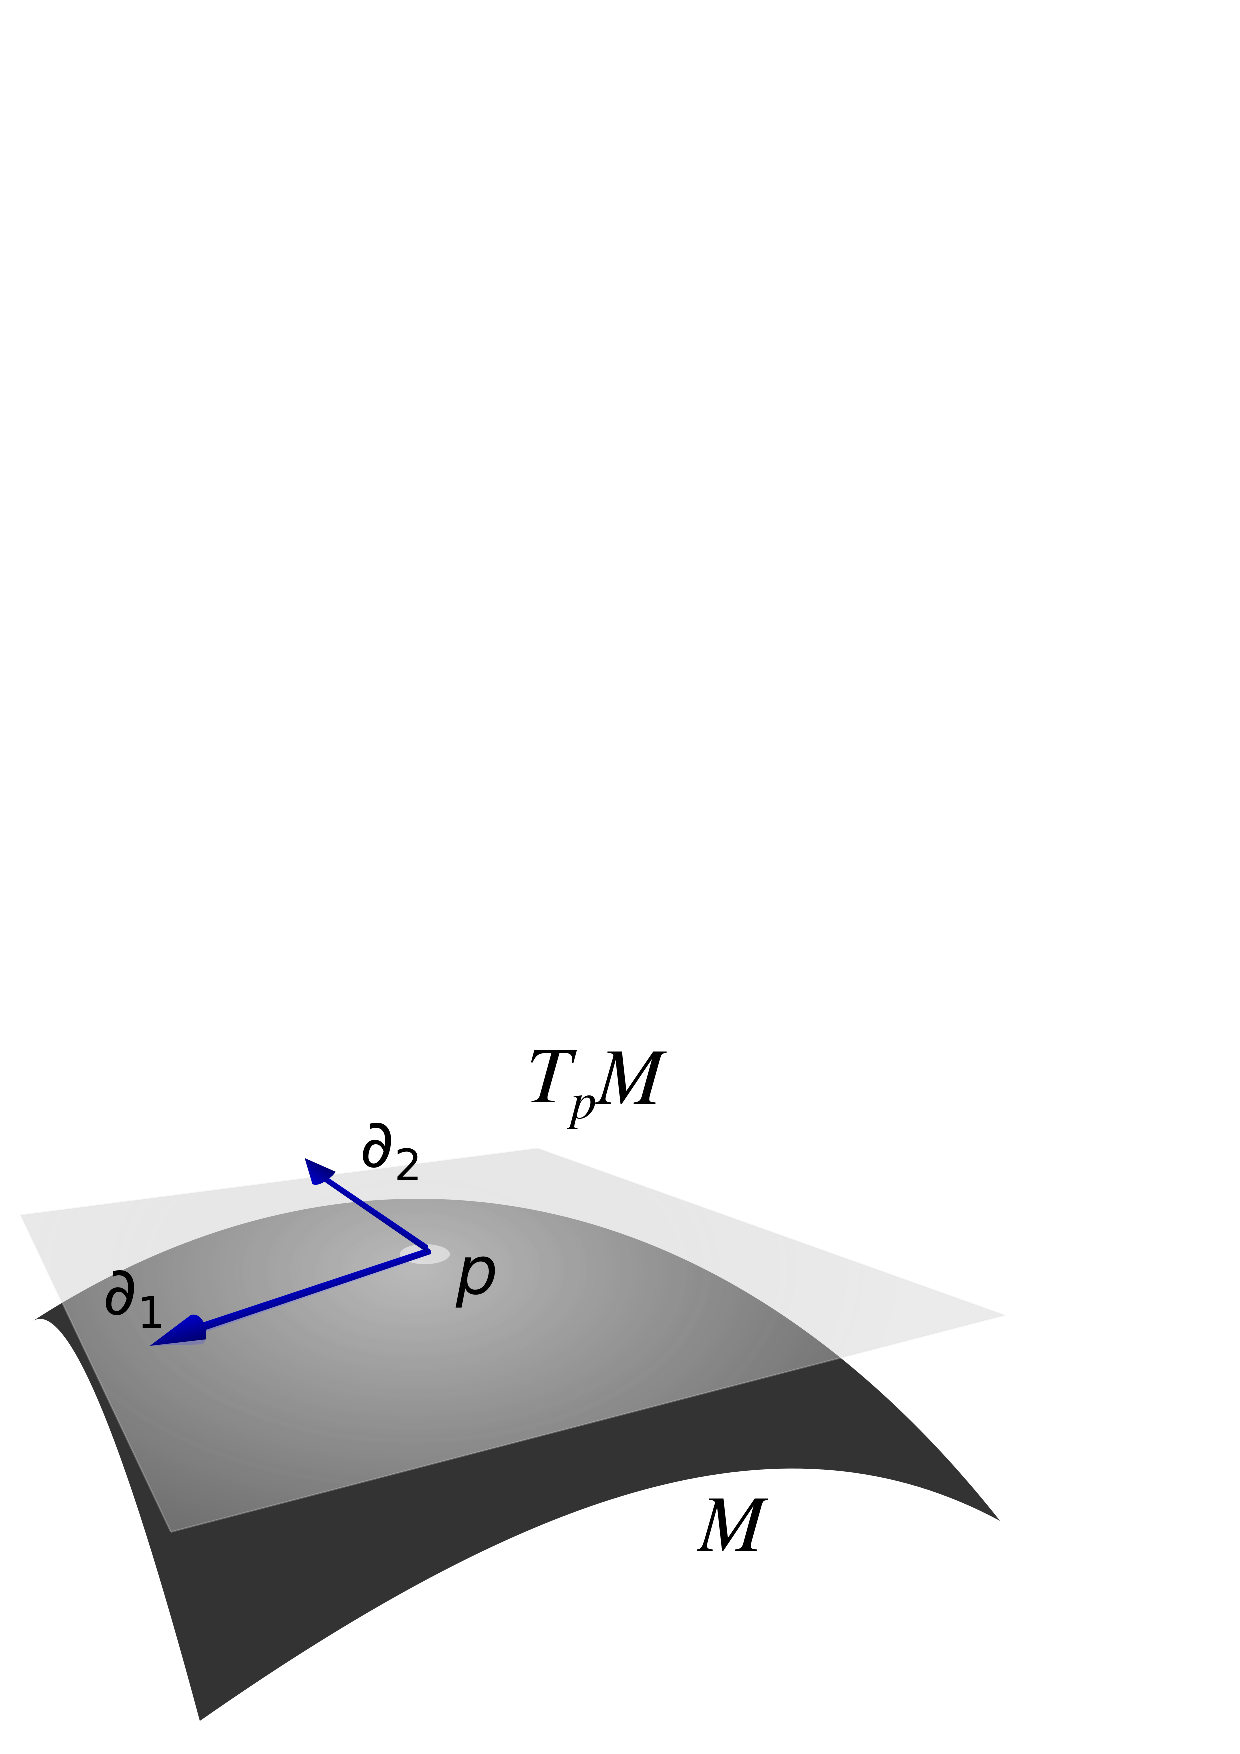
\includegraphics[scale=0.3]{Tangentialvektor.png}
%\end{center}

\begin{figure}[h!]
	\centering
	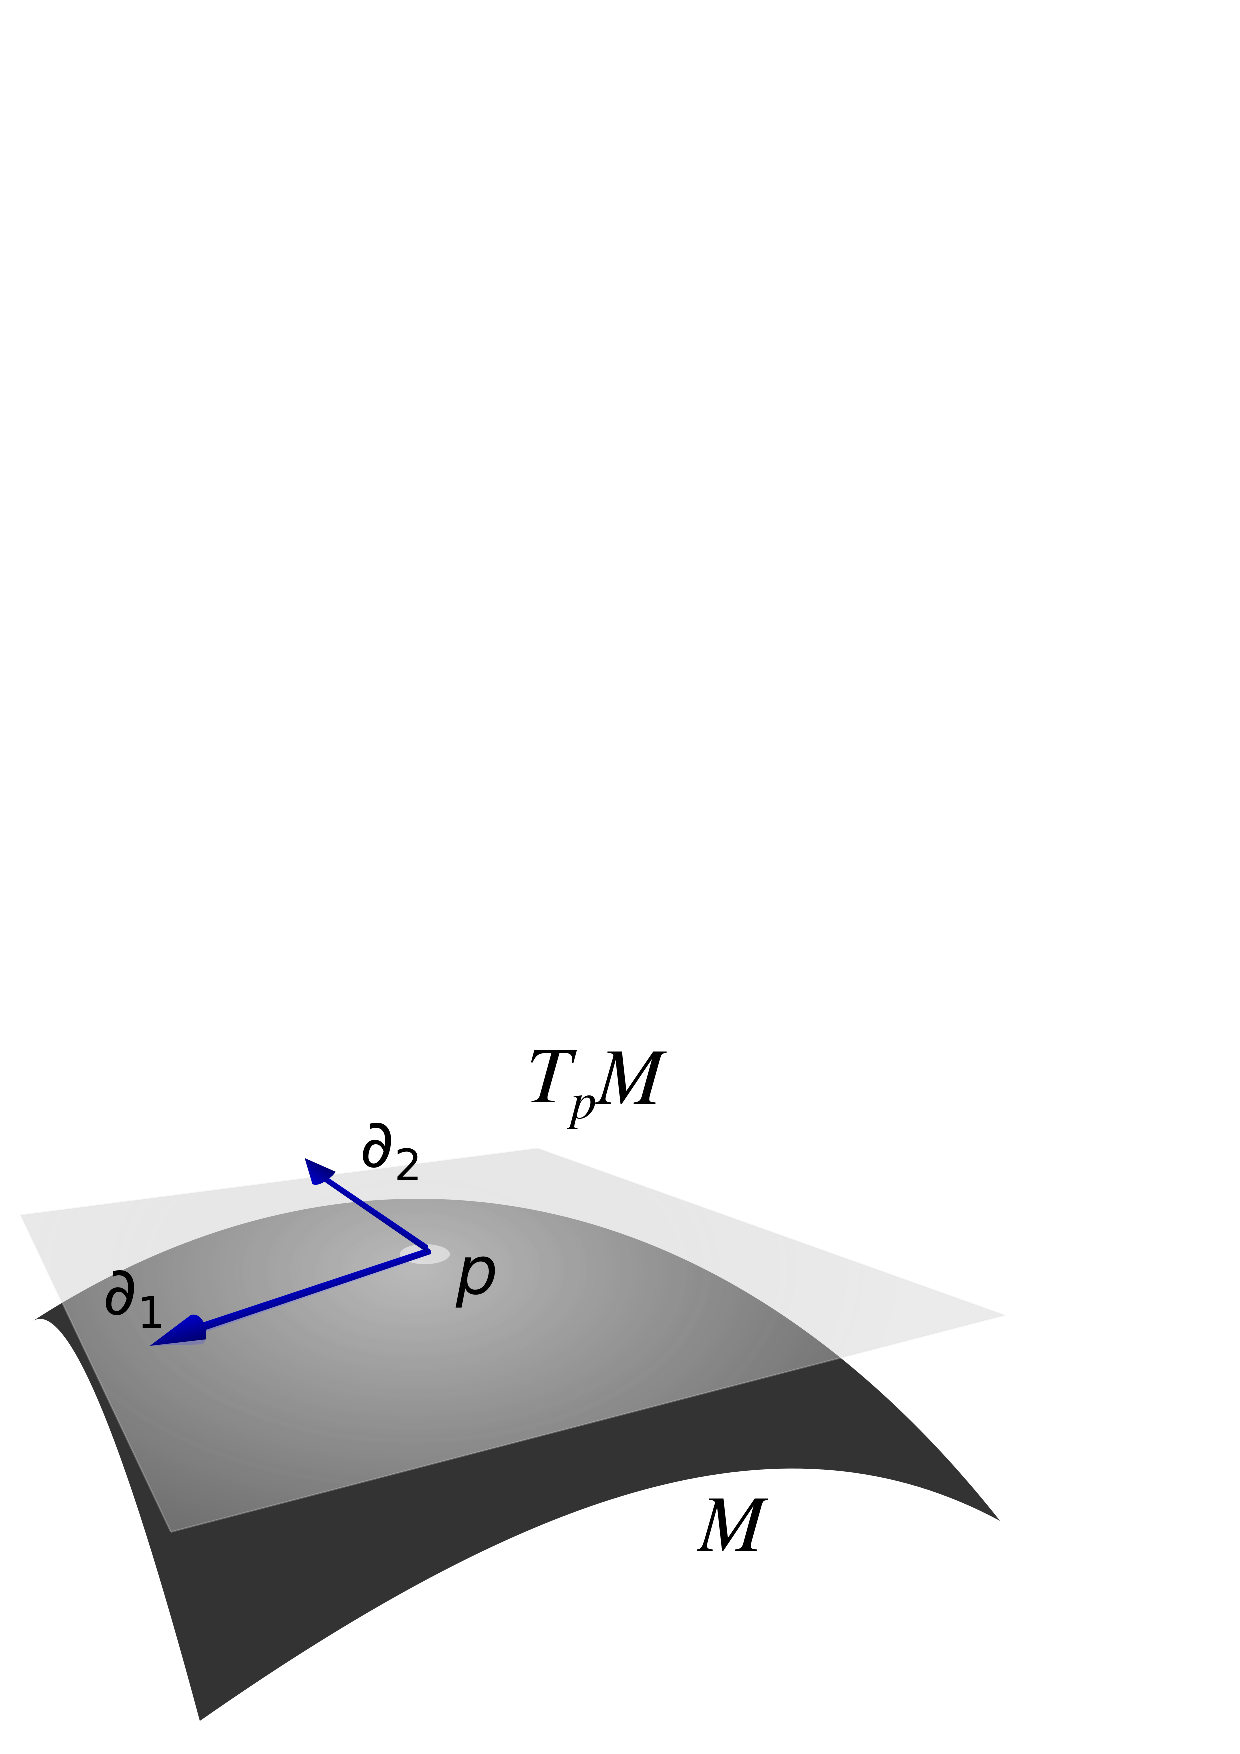
\includegraphics[scale=0.3]{Tangentialvektor.png}
	\caption{A visualisation of the tangent plane $T_{p} (M)$ to a manifold $M$ in 2 dimensions.}
\end{figure}

The vectors in the tangent space are what we will identify as contravariant vectors \cite{hartle, carroll}. Due to using the coordinate basis we can think of such vectors as being differential operators on the tangent plane. Thus we see that a vector can be represented as a sum of its coordinates \(A^{\mu}\) and the differential operators at the point \(\partial_{\nu}\). That is

\begin{equation} \label{contravariant}
	\vec{A} = A^{\mu} \partial_{\mu} = A^{0} \partial_{0} + A^{1} \partial_{1} + A^{2} \partial_{2} + A^{3} \partial_{3} .
\end{equation} 

We can now introduce another set of vectors at a point \(p\) on the manifold. If we consider the set of linear maps from the tangent space to the real numbers, \(\omega : T_{p} (M) \rightarrow \mathbb{R}\), we can construct the dual vector space of the tangent space to the manifold at a point \(p\), \(T_{p}^{*} (M)\) \cite{carroll}. We choose the basis of this vector space, \(\hat{e}^{\nu}\) such that \cite{carroll, hartle} 

\begin{equation} \label{cotangent-basis}
	\hat{e}^{\nu} \, \, \hat{e}_{\mu} = \df{\nu} (\partial_{\mu}) = \frac{\partial x^{\nu}}{\partial x^{\mu}} = \delta^{\nu}_{\mu} .
\end{equation} 

From this basis, \(\hat{e}^{\mu} = \df{\mu}\), we can construct any general linear map from vectors in the tangent space to the real numbers. Thus we can give an expression for the covectors much like \eqref{contravariant} \cite{carroll}

\begin{equation} \label{covarient}
	\vec{\omega} = \omega_{\mu} \df{\mu} = \omega_0 \df{0} + \omega_1 \df{1} +\omega_2 \df{2} +\omega_3 \df{3} .
\end{equation} 

Explicitly, by choosing the bases as we have, the linear mapping \(\omega : T_{p} (M) \rightarrow \mathbb{R}\) must be the same as the standard euclidean inner product \cite{hartle}. That is, if we take the contraction of a vector and a covector \(A^{\mu} \omega_{\mu}\) we obtain the sum of the product of the components of the vector and covector \cite{hartle}

\begin{equation} \label{inner}
	\begin{aligned}
	\omega_{\mu} \df{\mu} (A^{\nu} \partial_{\nu}) &= \omega_{\mu} A^{\nu} (\df{\mu} \partial_{\nu}) = \omega_{\mu} A^{\nu} \delta^{\mu}_{\nu} = \omega_{\mu} A^{\mu} \\
	&= \omega_0 A^0 + \omega_1 A^1 + \omega_2 A^2 + \omega_3 A^3 \in \mathbb{R} .
	\end{aligned}
\end{equation} 

From here on in we will refer to a vectors components, \(A^{\mu}\), as the vector itself, and the components of a covector as the covector itself. The implicit understanding here is that we are using the coordinate basis, and that therefore vectors at any point in the manifold will always be defined in the way given above.

We are now prepared to define the objects which we will use most throughout our discussion of General Relativity, tensors. First we recall a theorem from linear algebra.

\begin{thm} \label{dual}
In a finite dimensional vector space \(V\) with a dual space \(V^{*}\) the dual of the dual space \(V^{**}\) is isomorphic to the original space \(V\). {\normalfont\cite{szekeres}}
\end{thm}

Thus, due to \ref{dual}, we see that in addition to a covector acting on a vector as a linear operator we can consider the converse to be true: a vector can act on a covector as a linear operator. This is generally the case with a tensor: a tensor will take as an input vectors and covectors and map them to the real numbers. Thus we can define a tensor \(T\) as follows \footnote{In this definition we state that tensors map to the real numbers, however to be more correct we would have to say that tensors map to the field that the manifold is constructed over. Here we will always take this to be \(\mathbb{R}\).} \cite{carroll, szekeres}
\begin{equation} \label{tensor-def}
	T : \underbrace{T_{p}^{*}(M) \times \cdots \times T_{p}^{*}(M)}_{p \,\, \text{times}} \times \underbrace{T_{p}(M) \times \cdots \times T_{p}(M)}_{q \,\, \text{times}} \rightarrow \mathbb{R} .
\end{equation} 

In the above expression we take \(\times\) to be the Cartesian product: that is the above expression takes as an input ordered pairs of \(p\) covectors and \(q\) vectors.

We now can define the type of a tensor: the tensor above is of type \( \left[ \begin{smallmatrix} p \\ q \end{smallmatrix} \right] \). We will call the \(p\) covectors we input as \(p\) ``up'' indices and the \(q\) vectors ``down'' indices. That is, the tensor above would be given as \(T\indices{^{\sigma_{1}}^\cdots^{\sigma_{p}}_{\alpha_{1}}_\cdots_{\alpha_{q}}}\) \cite{carroll}. In this way we can see that vectors are a type \( \left[ \begin{smallmatrix} 1 \\ 0 \end{smallmatrix} \right] \) tensor and covectors are of type \( \left[ \begin{smallmatrix} 0 \\ 1 \end{smallmatrix} \right] \). We will define scalars to be of type \( \left[ \begin{smallmatrix} 0 \\ 0 \end{smallmatrix} \right] \) \cite{szekeres}. 

Finally we can introduce the tensor product, \(\otimes\). 
The tensor product is a linear product of tensors, that is if we add a tensor \(T\) of type \( \left[ \begin{smallmatrix} p \\ q \end{smallmatrix} \right] \) and a tensor \(S\) of type \( \left[ \begin{smallmatrix} r \\ s \end{smallmatrix} \right] \) we form \(T \otimes S\) of type \( \left[ \begin{smallmatrix} p+r \\ q+s \end{smallmatrix} \right] \). In terms of indices we have that the tensor product is like multiplication between tensors: if \(T = T^{\lambda \sigma}\) and \(S = S_{\mu \nu}\) then \(T \otimes S = T^{\lambda \sigma} S_{\mu \nu}\) \cite{carroll, szekeres}.

\subsection{Index Rules}

Before we continue it is worth summarizing the rules for index calculus with tensors. We use the Einstein summation convention throughout the text, where any repeated index (one upper and one lower) is summed over. That is, in an \(n\) dimensional space we would have 
\begin{equation} \label{summation-convention}
	v^i w_i = \sum_{i=0}^{n-1} v^i w_i
\end{equation}
assuming that we are using zero indexes. We can now introduce several other operations on tensors.
\begin{itemize}
	\item Contraction is an operation which maps a \( \left[ \begin{smallmatrix} p \\ q \end{smallmatrix} \right] \) type tensor to a \( \left[ \begin{smallmatrix} p-1 \\ q-1 \end{smallmatrix} \right] \) tensor by setting two of the indices equal to each other and summing them. That is if we have a tensor \( K\indices{^\mu^\lambda^\sigma_\alpha_\gamma_\phi}\) and we contract the \(\phi\) and \(\sigma\) indices we will obtain a new tensor, of type \( \left[ \begin{smallmatrix} 2 \\ 2 \end{smallmatrix} \right] \) \cite{carroll}
\end{itemize}
\begin{equation} \label{contration}
	K\indices{^\mu^\lambda^\sigma_\alpha_\gamma_\sigma} = \,\,\, L\indices{^\mu^\lambda_\alpha_\gamma} .
\end{equation}
\begin{itemize}
	\item[] In the case of a matrix this operation is the same as the trace. In order to contract over two upper or two lower indices we will need the metric tensor, which we will introduce in the next section.
	\item A tensor is considered to be symmetric in some of its indices if we can exchange their order and still obtain the same tensor. As an example, if \(S\indices{^\mu^\nu_\sigma_\alpha}\) is symmetric in the upper indices then \(S\indices{^\mu^\nu_\sigma_\alpha} = S\indices{^\nu^\mu_\sigma_\alpha}\) \cite{carroll}.
	\item Similarly a tensor is antisymmetric if when we exchange two indices we obtain the same tensor, but the tensor also changes sign. That is \(S\indices{^\mu^\nu_\sigma_\alpha} = -S\indices{^\nu^\mu_\sigma_\alpha}\).
	\item Given a tensor which is not symmetric we can create a symmetric tensor from it in any indices we wish. To do so we sum all permutations of the indices we are symmetrizing and divide by the number of terms in the sum. We will make clear which indices we are symmetrizing by surrounding them with round brackets \cite{carroll}
\end{itemize}
\begin{equation} \label{tensor-symmetrize}
	T\indices{_{(\mu_1 \mu_2 \cdots \mu_n)}_\rho^\sigma} = \frac{1}{n!} (T \indices{_{\mu_1}_{\mu_2}_{\cdots}_{\mu_n}_\rho^\sigma }
	+ \text{sum over permutations of indices}).
\end{equation}
\begin{itemize}
	\item In a similar way we can antisymmetrize a tensor in some of its indices using the same procedure, but alternating the sign of the terms in the sum over the permutations \cite{carroll}. We denote this by surrounding the relevant indices with square brackets.
\end{itemize}
\begin{equation} \label{tensor-antisymmetrize}
	T\indices{_{[\mu_1 \mu_2 \cdots \mu_n]}_\rho^\sigma} = \frac{1}{n!} (T \indices{_{\mu_1}_{\mu_2}_{\cdots}_{\mu_n}_\rho^\sigma }
+ \text{alternating sum over permutations of indices}) .
\end{equation}
\section{The Metric Tensor}

We now can define a new object on a manifold: the metric tensor \(g_{\mu \nu}\). This tensor is the ``star'' of General Relativity, as we will see in the subsequent discussion. From allowing us to perform calculations on the indices to allowing us to define the curvature of spacetime and eventually appearing in the all important Einstein Equation, the metric is omnipresent \cite{carroll, szekeres, cheng}.

We define the metric as being a type \( \left[ \begin{smallmatrix} 0 \\ 2 \end{smallmatrix} \right] \) tensor which takes two vectors as an input and gives back a separation between them
\begin{equation} \label{line-el}
	ds^2 = g_{\mu \nu} \df{\mu} \df{\nu} .
\end{equation}

Thus the metric supplies the idea of an inner product between two vectors, as opposed to a vector and a covector \cite{hartle}

\begin{equation} \label{inner-metric}
	g(\vec{A}, \vec{B}) = \vec{A} \cdot \vec{B} = g_{\mu \nu} A^{\mu} B^{\nu} .
\end{equation} 

We can now see how the metric must be used to raise and lower indices: in order for the inner product to work like \eqref{inner} we must have that the metric allows us to raise an index

\begin{equation} \label{raise}
	A_{\mu} = g_{\mu \nu} A^{\nu} .
\end{equation}

If we now introduce the inverse metric \(g^{\mu \nu}\) which is defined to be the tensor such that \cite{carroll}:
\begin{equation} \label{inverse-metric}
	g^{\mu \nu} g_{\nu \sigma} = g_{\lambda \sigma} g^{\lambda \mu} = \delta^{\mu}_{\sigma} \,\, ,
\end{equation}
\noindent we can then use the inverse metric to lower an index
\begin{equation} \label{lower}
	A^{\mu} = g^{\mu \nu} A_{\nu} .
\end{equation}

One of the most important features of relativistic theory is that \(ds^2\) must be a relativistic invariant, that is, no matter what choice of coordinates \(ds^2\) must always take the same value for the same spacetime events. We will see this is due to how tensors transform, with vectors transforming in such a way as to cancel the transformation of the matrix.

In the 4 dimensional spacetime of general relativity the metric takes the form of a position dependent symmetric 4 by 4 matrix with one negative and three positive eigenvalues 
\footnote{We can also take this to be one positive and three negative eigenvalues. The choice between the two is just convention.}. 
Explicitly, this is

\begin{equation} \label{metric-matrix}
	g_{\mu \nu} (x^{\sigma}) \equiv
	\begin{pmatrix} 
	g_{00} (x^{\sigma}) & g_{01} (x^{\sigma}) & g_{02} (x^{\sigma}) & g_{03} (x^{\sigma}) \\
	g_{01} (x^{\sigma}) & g_{11} (x^{\sigma}) & g_{12} (x^{\sigma}) & g_{13} (x^{\sigma}) \\
	g_{02} (x^{\sigma}) & g_{12} (x^{\sigma}) & g_{22} (x^{\sigma}) & g_{23} (x^{\sigma}) \\
	g_{03} (x^{\sigma}) & g_{13} (x^{\sigma}) & g_{23} (x^{\sigma}) & g_{33} (x^{\sigma}) 
\end{pmatrix} .
\end{equation}

\noindent In the special relativistic case where spacetime is flat this reduces to the Minkowski metric

\begin{equation} \label{metric-sr}
	\eta_{\mu \nu} (x^{\sigma}) \equiv
	\begin{pmatrix} 
	-1 & 0 & 0 & 0 \\
	0 & 1 & 0 & 0 \\
	0 & 0 & 1 & 0 \\
	0 & 0 & 0 & 1 
	\end{pmatrix} .
\end{equation}

In keeping with the equivalence principle it is also possible to transform the metric at any point such that is it the same as the Minkowski metric \(\eta_{\mu \nu}\) and that the first order partial derivatives vanish \cite{carroll}.

\section{Covariant Differentiation and the Connection}

In order to understand how to perform differentiation on the manifold we first need to understand how tensors transform from one coordinate system to another in general.

\noindent If we wish to switch from one set of coordinates $x^{\mu}$ to a new set of coordinates $x^{\mu^\prime}$. We define the matrix of transformation between the coordinates for a vector as \cite{cheng}

\begin{equation} \label{vector-transform}
	A^{\mu} \rightarrow A^{\mu^\prime} = \frac{\partial x^{\mu^\prime}}{\partial x^{\mu}} A^{\mu} .
\end{equation}

For a covector we have \cite{cheng}
\begin{equation} \label{covector-transform}
	A_{\mu} \rightarrow A_{\mu^\prime} = \frac{\partial x^{\mu}}{\partial x^{\mu^\prime}} A_{\mu} .
\end{equation}

Now we can define the transformation for an arbitrary tensor \footnote{We can consider this tensor transformation as another way of defining tensors, that is that they are objects which transform linearly under coordinate transformations.} \cite{carroll}
\begin{equation} \label{tensor-transform}
	T\indices{^{\mu_1}^{\cdots}^{\mu_k}_{\nu_1}_{\cdots}_{\nu_l}} \rightarrow T\indices{^{\mu_1^\prime}^{\cdots}^{\mu_k^\prime}_{\nu_1^\prime}_{\cdots}_{\nu_l^\prime}}
	= \frac{\partial x^{\mu_1^\prime}}{\partial x^{\mu}} \cdots \frac{\partial x^{\mu_k^\prime}}{\partial x^{\mu_k}} \frac{\partial x^{\nu_1}}{\partial x^{\nu_1^\prime}} \cdots 
	\frac{\partial x^{\nu_l}}{\partial x^{\nu_l^\prime}}
	T\indices{^{\mu_1}^{\cdots}^{\mu_k}_{\nu_1}_{\cdots}_{\nu_l}} .
\end{equation}

Now we can consider partial derivatives. The partial derivative operator is a covector, as shown in \eqref{coordinate-basis}, and transforms in the same way as any other covector given in \eqref{covector-transform}. However, when we apply the derivative to a vector and then attempt to change coordinates the result does not follow the rules. To see this consider $\partial_{\nu^\prime} A^{\mu^\prime}$ the derivative of a vector field. Use the definition \eqref{vector-transform} and differentiate on both sides \cite{cheng}
\begin{equation} \label{partial-transform}
\begin{aligned}
	\partial_{\nu^\prime} A^{\mu^\prime} &= \frac{\partial}{\partial x^{\nu^\prime}} \left(\frac{\partial x^{\mu^\prime}}{\partial x^{\rho}} A^{\rho}\right) \\
	&= \frac{\partial x^{\lambda}}{\partial x^{\nu^\prime}} \frac{\partial x^{\mu^\prime}}{\partial x^{\rho}} (\partial_{\lambda} A^{\rho}) + \frac{\partial^2 x^{\mu^\prime}}{\partial x^{\nu^\prime} \partial x^{\rho}} A^{\rho}
\end{aligned}
\end{equation}
which is not the same as the tensor transformation law given in \eqref{tensor-transform}.

This discrepancy is due to the position dependent transformation of tensors. Since on an arbitrary manifold the basis vectors of the tangent plane at a point are dependent on the choice of coordinate system, a tensor defined at one point will not necessarily be the same at another point \cite{cheng}.

In order to solve this problem we must introduce a new type of derivative which will transform as we expect under coordinate transformations. This is the covariant derivative. In order to find the covariant derivative we must first list several of the properties we will expect it to have \cite{carroll}.

\begin{itemize}
	\item Linearity: \(\nabla (T + S) = \nabla T + \nabla S\) .
	\item Obeys the product rule: \(\nabla (T \otimes S) = (\nabla T) \otimes S + T \otimes (\nabla S)\) .
	\item Commutes with the contraction operation: \(\nabla_{\mu} (S\indices{^\lambda_\lambda_\rho}) = (\nabla S)\indices{_\mu^\lambda_\lambda_\rho}\) .
	\item Like the partial derivative it maps a \( \left[ \begin{smallmatrix} r \\ s \end{smallmatrix} \right] \) type tensor to a \( \left[ \begin{smallmatrix} r \\ s+1 \end{smallmatrix} \right] \) type tensor.
	\item For a scalar, the covariant derivative is the same as a the partial derivative \(\nabla_{\mu} \phi = \partial_{\mu} \phi\).
\end{itemize}

In order for the operation to follow the product rule we will require it to be the same as the partial derivative plus an additional linear correction term \cite{carroll}. In order to do this we introduce a new linear term in the derivative, called the connection coefficients, which make the transformation of a derivative occur in the tensorial way. These coefficients are viewed as a matrix for each of the coordinate functions, that is \((\Gamma_{\mu})\indices{^\rho_\sigma}\) \cite{carroll}. We will drop the use of the brackets and understand that \(\Gamma^{\nu}_{\mu \sigma}\) has the same meaning. The covariant derivative of a vector will now be
\begin{equation} \label{co-deriv}
	\nabla_{\mu} V^{\nu} = \partial_{\mu} V^{\nu} + \Gamma^{\nu}_{\mu \sigma} V^{\sigma} .
\end{equation}

The transformation of this expression is designed to be tensorial, and as such the connection coefficients will not transform in a tensorial way but will transform so as to make the overall transformation tensorial. The transformation of the coefficients will be as follows \cite{carroll}: 

\begin{equation} \label{connection-transform}
	\Gamma^{\nu}_{\mu \sigma} \rightarrow \Gamma^{\nu'}_{\mu' \sigma'} = \frac{\partial x^{\mu}}{\partial x^{\mu'}} 
	\frac{\partial x^{\sigma}}{\partial x^{\sigma'}} \frac{\partial x^{\nu'}}{\partial x^{\nu}} \Gamma^{\nu}_{\mu \sigma} +
	\frac{\partial x^{\mu}}{\partial x^{\mu'}} \frac{\partial x^{\sigma}}{\partial x^{\sigma'}} \frac{\partial^2 x^{\nu'}}{\partial x^{\mu} \partial x^{\sigma}}
	.
\end{equation}

This will now correct for the second term in the expansion of the partial derivative of a vector, making it tensorial. In order to find the covariant derivative of a covector we first consider the derivative of the scalar \(\omega_{\mu} A^{\mu}\) \cite{carroll}. The definition of the covariant derivative given above is only for vectors, however it is reasonable to assume that the covariant derivative for a covector will be similar. Thus we introduce a new coefficient, which we will call \(\xi^{\sigma}_{\mu \lambda}\) for now, and covariantly differentiate \(\omega_{\mu} A^{\mu}\):

\begin{equation} \label{covar-deriv}
	\begin{aligned}
		\nabla_{\mu} (\omega_{\lambda} A^{\lambda}) &= (\nabla_{\mu} \omega_{\lambda}) A^{\lambda} + \omega_{\lambda} (\nabla_{\mu} A^{\lambda}) \\
		&= (\partial_{\mu} \omega_{\lambda}) A^{\lambda} + \xi^{\sigma}_{\mu \lambda} \omega_{\sigma} A^{\lambda}
		+ \omega_{\lambda} (\partial_{\mu} A^{\lambda}) + \omega_{\lambda} \Gamma^{\lambda}_{\mu \rho} A^{\lambda} .
	\end{aligned}
\end{equation}

Since this is the covariant derivative of a scalar, we must have that it is equal to the partial derivative. Thus we can also write:

\begin{equation} \label{covar-partial}
	\begin{aligned}
		\nabla_{\mu} (\omega_{\lambda} A^{\lambda}) &= \partial_{\mu} (\omega_{\lambda} A^{\lambda}) \\
		&= (\partial_{\mu} \omega_{\lambda}) A^{\lambda} + \omega_{\lambda} (\partial_{\mu} A^{\mu}) .
	\end{aligned}
\end{equation}

From here we can obviously see that \(\xi^{\sigma}_{\mu \lambda} = - \Gamma^{\lambda}_{\mu \rho}\) and thus for a covector the covariant derivative is given by \cite{carroll}

\begin{equation} \label{covar-diff}
	\nabla_{\mu} \omega_{\nu} = \partial_{\mu} \omega_{\nu} - \Gamma^{\lambda}_{\mu \nu} \omega_{\lambda} .
\end{equation}

We can now define the covariant derivative for any tensor, once again by considering it as a product of vectors and covectors, thus we see \cite{carroll}

\begin{equation} \label{tensor-diff}
	\begin{aligned}
	\nabla_{\sigma} T\indices{^{\mu_1}^\cdots^{\mu_k}_{\nu_1}_\cdots_{\nu_l}} = \partial_{\sigma} T\indices{^{\mu_1}^\cdots^{\mu_k}_{\nu_1}_\cdots_{\nu_l}}
	&+ \Gamma^{\mu_1}_{\sigma \lambda} T\indices{^{\mu_1}^\cdots^{\mu_k}_{\nu_1}_\cdots_{\nu_l}} + \, \cdots \, + \Gamma^{\mu_k}_{\sigma \lambda} T\indices{^{\mu_1}^\cdots^{\mu_k}_{\nu_1}_\cdots_{\nu_l}} \\
	&- \Gamma^{\lambda}_{\sigma \nu_1} T\indices{^{\mu_1}^\cdots^{\mu_k}_{\nu_1}_\cdots_{\nu_l}} - \, \cdots \, - \Gamma^{\lambda}_{\sigma \nu_l} T\indices{^{\mu_1}^\cdots^{\mu_k}_{\nu_1}_\cdots_{\nu_l}} .
	\end{aligned}
\end{equation}

Now we can introduce the specific connection we will use in General Relativity, the Levi-Civita connection \cite{carroll, szekeres}. With this connection we demand the following things:

\begin{itemize}
	\item The connection coefficients are torsion free, that is \(\Gamma^{\lambda}_{\mu \nu} = \Gamma^{\lambda}_{\nu \mu}\).
	\item Metric compatibility, that is \(\nabla_{\mu} g_{\nu \sigma} = 0\).
\end{itemize}

The Levi-Civita connection is the only connection which will have both such properties. This is known as the fundamental theorem of Riemannian geometry. From here we can derive an expression for the connection coefficients for the Levi-Civita connection in terms of the metric. If we consider the covariant derivative of the metric \(\nabla_{\rho} g_{\mu \nu}\) and permute the three indices \cite{carroll, cheng}:

\begin{equation} \label{metric-deriv}
	\begin{aligned}
		\nabla_{\rho} g_{\mu \nu} &= \partial_{\rho} g_{\mu \nu} - \Gamma^{\lambda}_{\rho \mu} g_{\lambda \nu} - \Gamma^{\lambda}_{\rho \nu} g_{\mu \nu} = 0 ,\\
		\nabla_{\mu} g_{\nu \rho} &= \partial_{\mu} g_{\nu \rho} - \Gamma^{\lambda}_{\mu \nu} g_{\lambda \rho} - \Gamma^{\lambda}_{\mu \rho} g_{\nu \lambda} = 0 ,\\
		\nabla_{\nu} g_{\rho \mu} &= \partial_{\nu} g_{\rho \mu} - \Gamma^{\lambda}_{\nu \rho} g_{\lambda \mu} - \Gamma^{\lambda}_{\nu \mu} g_{\rho \lambda} = 0 .
	\end{aligned}
\end{equation}

Now if we take the first equation and subtract the second and third from it, then multiply by the inverse metric we will obtain the desired expression for the coefficients \cite{carroll}

\begin{equation} \label{christ-def}
	\Gamma^{\lambda}_{\mu \nu} = \frac{1}{2} g^{\lambda \sigma} \left( \partial_{\mu} g_{\nu \sigma} + \partial_{\nu} g_{\sigma \mu} - \partial_{\sigma} g_{\mu \nu} \right) .
\end{equation}

This is the expression we will use as the definition of the connection coefficients.

\section{Parallel Transport}

In order to understand the curvature on the manifold we first need a new concept called parallel transport. Parallel transport is the operation of moving a tensor along a path on the manifold in such a way that the covariant derivative of the tensor along the path is zero. That is any changes to the tensor as a result of moving along the curve are due to the structure of space, not due to the tensor itself changing.

If we consider a curve \(\gamma\) on the manifold \(M\) given by a parameterization \(x^{\mu} (\lambda)\) with \(\lambda\) an affine parameter \footnote{An affine parameter is a parameter which is related to the proper time \(\tau\) by real coefficients \(a\) and \(b\) in the form \( \lambda = a \tau + b\). We will introduce the proper time soon.} and with the tangent vector to the curve of \(T^{\mu} = \frac{d x^{\mu}}{d \lambda}\) we can define the directional covariant derivative to be \cite{carroll}

\begin{equation} \label{directional}
	\frac{D}{d \lambda} = \frac{d x^{\mu}}{d \lambda} \nabla_{\mu} .
\end{equation}

We now say that a vector \(V^{\mu}\) is parallel transported along \(\gamma\) when

\begin{equation} \label{parallel}
	\frac{D V^{\mu}}{d \lambda} = 0 .
\end{equation}

This can be rephrased as \cite{carroll}

\begin{equation} \label{vector-parallel}
	\frac{d}{d \lambda} V^{\mu} + \Gamma^{\mu}_{\sigma \rho} \frac{d x^{\sigma}}{d \lambda} V^{\rho} = 0 .
\end{equation}

We are now ready to define one of the key ideas in general relativity: a geodesic path. A geodesic is the shortest path between two points, and brings the idea of a straight line in flat space into the curved spaces we will use in relativity. In keeping with this idea, we will define a geodesic to be a path for which the tangent vector \(T^{\mu}\) is parallel transported along the path \cite{carroll}. That is

\begin{equation} \label{geodesic0}
	\frac{D}{d \lambda} T^{\mu} = \frac{D}{d \lambda} \frac{d x^{\mu}}{d \lambda} = 0 .
\end{equation}

Inserting this into \eqref{vector-parallel} gives the standard geodesic equation: 

\begin{equation} \label{geodesic}
	\frac{d^2 x^{\mu}}{d \lambda^2} + \Gamma^{\mu}_{\rho \sigma} \frac{d x^{\rho}}{d \lambda} \frac{d x^{\sigma}}{d \lambda} = 0 .
\end{equation}

These results can also be obtained using variational methods \cite{carroll}, however we will not reproduce such proofs here. 

\section{World Lines}

A world line is a path \(\gamma\) as measured on the spacetime manifold between events. We can then define the type of the world line by considering what physical phenomena can occur on that path through spacetime. Since the speed of light is the highest attainable speed we will find that spacetime intervals can be divided into cases where normal objects can traverse the distance in spacetime, only light can traverse the distance in spacetime, or no physical phenomena can travserse the distance \cite{cheng, hartle, carroll}. 

We have, for the tangent vector \(T^{\mu}\) to a curve \(\gamma\) with parameter \(\lambda\) the following three possibilities:

\begin{itemize}
	\item If \(g_{\mu \nu} T^{\mu} T^{\nu} = 0\) then the curve is light-like or null. Paths such as these are the paths which light travels along.
	\item If \(g_{\mu \nu} T^{\mu} T^{\nu} < 0\) then the curve is time-like. These paths are the paths which objects with mass travel along, at less than the speed of light.
	\item If \(g_{\mu \nu} T^{\mu} T^{\nu} > 0\) then the curve is space-like. These paths are impossible for any object to travel along, and thus are completely physically disparate.
\end{itemize}

If we choose the parameterization of the curve \(\gamma\) such that \(g_{\mu \nu} T^{\mu} T^{\nu} = -1\) then the parameter is the proper time for an object, \(\tau\). This is the time measured by an observer moving on the path \(\gamma\) through spacetime \cite{cheng}.

For a timelike path we can now rewrite the geodesic equation \eqref{geodesic} in terms of the four-velocity \cite{carroll} \(U^{\mu} = dx^{\mu} / d \tau\)

\begin{equation} \label{geodesic-timelike}
	U^{\nu} \nabla_{\nu} U^{\mu} = 0 .
\end{equation}

\section{Riemann Curvature Tensor}

In order to measure the curvature of a manifold we need a new tensor which measures the change of a vector moving on the manifold around a closed loop. We choose a closed loop in order to see how the manifold varies from flat space: if the vector is unchanged by its journey around the loop then we should be in flat space \cite{cheng, carroll}.

For an arbitrary vector \(V^{\mu}\) we have that the Riemann curvature tensor is defined as \cite{carroll}

\begin{equation} \label{riemann}
	(\nabla_{\phi} \nabla_{\sigma} - \nabla_{\sigma} \nabla_{\phi}) V^{\mu} = R\indices{^\mu_\nu_\phi_\sigma} V^{\nu} .
\end{equation}

This definition of the Riemann curvature tensor is only true for connections which have torsion free coefficients \cite{lovelock}.

While we will not prove this definition, we can give some motivation for how it works. The covariant derivative effectively measures how much a vector moves away from a path on which it is parallel transported. On flat space, this deviation would be zero, and thus the curvature tensor would be zero. The terms involving the covariant derivative measure the change of a vector compared to its parallel transport in that direction. Thus by considering two different directions we can obtain the loop mentioned above. This also gives the condition that in flat space the tensor should be zero, as \(\nabla_{\phi} \nabla_{\sigma} - \nabla_{\sigma} \nabla_{\phi} = \partial_{\phi} \partial_{\sigma} - \partial_{\sigma} \partial_{\phi} = 0\) in flat space \cite{cheng, carroll, woodhouse}.

If we now perform the computation in \eqref{riemann} with an arbitrary vector \(V^{\lambda}\) we can obtain an expression for the Riemann curvature tensor in terms of the connection coefficients \cite{carroll, woodhouse}. First consider \(\nabla_{\mu} \nabla_{\nu} V^{\lambda}\)

\begin{equation} \label{riemann-deriv}
	\begin{aligned}
		\nabla_{\mu} \nabla_{\nu} V^{\lambda} &= \nabla_{\mu} (\partial_{\nu} V^{\lambda} + \Gamma^{\lambda}_{\nu \sigma} V^{\sigma}) \\
		&= \partial_{\mu} \partial_{\nu} V^{\lambda} + (\partial_{\mu} \Gamma^{\lambda}_{\nu \sigma}) + \Gamma^{\lambda}_{\nu \sigma} \partial_{\mu} V^{\sigma}
		+ \Gamma^{\lambda}_{\mu \phi} (\partial_{\nu} V^{\phi} + \Gamma^{\phi}_{\nu \sigma} V^{\sigma}) - \Gamma^{\sigma}_{\mu \nu} (\partial_{\sigma} V^{\lambda}
		+ \Gamma^{\lambda}_{\phi \sigma})
	\end{aligned}
\end{equation}
now by exchanging \(\mu\) and \(\nu\) and using the properties of the connection we can find
\begin{equation} \label{riemann-deriv2}
	(\nabla_{\mu} \nabla_{\nu} - \nabla_{\nu} \nabla_{\mu}) V^{\lambda} = (\partial_{\mu} \Gamma^{\lambda}_{\nu \sigma} - \partial_{\nu}\Gamma^{\lambda}_{\mu \sigma} 
	+ \Gamma^{\lambda}_{\mu \lambda} \Gamma^{\phi}_{\nu \sigma} - \Gamma^{\lambda}_{\nu \lambda} \Gamma^{\phi}_{\mu \sigma}) V^{\sigma} .
\end{equation}

Thus we can give an expression for the Riemann curvature tensor in terms of the connection coefficients. This is the expression most commonly used to calculate the tensor 

\begin{equation} \label{riemann-christoffel}
	R\indices{^\rho_\sigma_\mu_\nu} = \partial_{\mu} \Gamma^{\rho}_{\nu \sigma} - \partial_{\nu}\Gamma^{\rho}_{\mu \sigma} 
	+ \Gamma^{\rho}_{\mu \lambda} \Gamma^{\lambda}_{\nu \sigma} - \Gamma^{\rho}_{\nu \lambda} \Gamma^{\lambda}_{\mu \sigma} .
\end{equation}

\subsection{Properties of the Riemann Curvature Tensor}

We will list some of the important properties of the Riemann curvature tensor. These are easier to see in the version of the tensor with 4 lower indices 

\begin{equation} \label{riemann-lower}
	R\indices{_\rho_\sigma_\mu_\nu} = g_{\rho \lambda} R\indices{^\lambda_\sigma_\mu_\nu} .
\end{equation}

\begin{itemize}
	\item Antisymmetry in the first two indices \(R\indices{_\rho_\sigma_\mu_\nu} = -R\indices{_\sigma_\rho_\mu_\nu}\) and in the last two indices \\ \(R\indices{_\rho_\sigma_\mu_\nu} = -R\indices{_\rho_\sigma_\nu_\mu}\).
	\item Symmetric when exchanging the first pair of indices with the second \(R\indices{_\rho_\sigma_\mu_\nu} = R\indices{_\mu_\nu_\rho_\sigma}\).
	\item The sum of the cyclic permutations of the last three indices is zero \(R\indices{_\rho_\sigma_\mu_\nu} + R\indices{_\rho_\mu_\nu_\sigma} + R\indices{_\rho_\nu_\sigma_\mu} = 0\)
\end{itemize}

From these properties it is possible to show that in \(n\) dimensional space the Riemann curvature tensor must have \(N\) independent components \cite{cheng}, where \(N\) is
\begin{equation}
	N = \frac{1}{12} n^2 (n^2 -1) .
\end{equation}

\begin{remark}
When \(n=1\) we have that \(N = 0\) and thus there can be no curvature for a line. For a surface however, with \(n=2\), we find that \(N=1\). This single independent component is related to the Gaussian curvature {\normalfont \cite{cheng, landau}} of a surface from classical differential geometry. We have that
\begin{equation}
	K = - \frac{R_{1212}}{|g_{\mu \nu}|}
\end{equation}
with \(|g_{\mu \nu}|\) being the determinant of the metric tensor and \(K\) the Gaussian curvature. With \(n=4\) we have 20 independent components of the Riemann curvature tensor.
\end{remark}

Finally another important property is the Bianchi identity

\begin{equation} \label{bianchi}
	\nabla_{\omega} R\indices{_\rho_\sigma_\mu_\nu} + \nabla_{\rho} R\indices{_\sigma_\omega_\mu_\nu} + \nabla_{\sigma} R\indices{_\omega_\rho_\mu_\nu} = 0 .
\end{equation}

We can also write this by using the antisymmetry properties of \(R\indices{_\rho_\sigma_\mu_\nu}\) as

\begin{equation} \label{bianchi2}
	\nabla_{[\omega} R\indices{_\rho_{\sigma ]}_\mu_\nu} = 0 .
\end{equation}

\subsection{Ricci Tensor}

If we now contract the first and third indices of the Riemann curvature tensor we can form the Ricci tensor \cite{carroll}

\begin{equation} \label{ricci-tensor}
	R\indices{_\mu_\nu} = R\indices{^\lambda_\mu_\lambda_\nu} .
\end{equation}

Due to our choice of the connection this is the only contraction of the Riemann curvature tensor which yields interesting results. All other contractions are either zero or related to the Ricci tensor \cite{carroll}. The Ricci tensor is also symmetric in its indices.

\subsection{Ricci Scalar}

If we now raise one of the indices of the Ricci tensor and then contract over the indices we will obtain the Ricci scalar

\begin{equation} \label{ricci-scalar}
	R = R\indices{^\mu_\mu} = g^{\mu \nu} R_{\mu \nu} .
\end{equation}

\subsection{Einstein Tensor}

We now can derive the Einstein tensor, which is the tensor we will use to describe the curvature of space in the Einstein equation. If we take the Bianchi identity \eqref{bianchi} and contract twice we will obtain a similar identity in terms of the Ricci tensor and scalar

\begin{equation} \label{bianchi-contract}
	\begin{aligned}
		g^{\nu \sigma} g^{\mu \lambda} (\nabla_{\lambda} R\indices{_\rho_\sigma_\mu_\nu} + \nabla_{\rho} R\indices{_\sigma_\lambda_\mu_\nu} + \nabla_{\sigma} R\indices{_\lambda_\rho_\mu_\nu}) &= 0  , \\
		\nabla^{\mu} R\indices{_\rho_\mu} - \nabla_{\rho} R + \nabla^{\nu} R\indices{_\rho_\nu} &= 0 .
	\end{aligned}
\end{equation}

\noindent Now if we define the Einstein tensor 
\begin{equation} \label{einstein-tensor}
	G\indices{_\mu_\nu} = R\indices{_\mu_\nu} - \frac{1}{2} R g_{\mu \nu}
\end{equation}
we can see that the contracted Bianchi identity must imply that \cite{cheng, carroll}
\begin{equation} \label{etensor0}
	\nabla^{\mu} G\indices{_\mu_\nu} = 0 .
\end{equation}

\section{The Energy Momentum Tensor}

The fundamental idea of General Relativity is that the curvature of spacetime is caused by the nearby mass and energy at that point \cite{hartle, carroll}. We now have the mathematical description of how the curvature of space is measured. Thus, we now need to develop an object to measure the amount of mass and energy near a point. This is the energy momentum tensor.

The energy momentum tensor is a type \( \left[ \begin{smallmatrix} 2 \\ 0 \end{smallmatrix} \right] \) symmetric tensor which measures the flux of four momentum \(p^{\mu}\) across a surface keeping one coordinate constant \cite{carroll}. In 3 dimensional flat space this would represent the forces pointing in three orthogonal directions along three orthogonal planes at a point \cite{cheng}.

In 4 dimensional general relativity we have to take into account energy as well, as due to the classic equation from special relativity for the rest energy of matter
\begin{equation} \label{ifweonlyhadoneequation}
	E = mc^2
\end{equation}
we can view energy as having a mass. Thus in the 4 dimensional case we take the energy momentum tensor to be in matrix form
\begin{equation} \label{e-m-tensor}
	T^{\mu \nu} = 
	\begin{pmatrix} 
		T^{00} & T^{01} & T^{02} & T^{03} \\ 
		T^{10} & T^{11} & T^{12} & T^{13} \\ 
		T^{20} & T^{21} & T^{22} & T^{23} \\ 
		T^{30} & T^{31} & T^{32} & T^{33} 
	\end{pmatrix} .
\end{equation}

We can now identify the components of this equation \cite{hartle, carroll}

\begin{itemize}
	\item \(T^{00}\) is the energy density at the point, which we will call \(\rho\). 
	\item \(T^{0i} = T^{i0}\) for the three spatial indices is the momentum density at the point.
	\item Terms on the diagonal \(T^{ii}\) give the spatial components of the pressure \(p_{i}\).
	\item All other off diagonal terms represent the sheering terms, that is forces on the planes not in the direction of the plane. These are created due to things like viscosities.
\end{itemize}

An example of this, and the one used most in modeling physical situations in general relativity is of the perfect fluid, which we will take to have an energy momentum tensor of \cite{carroll, hartle}
\begin{equation} \label{perfect-fluid}
	T^{\mu \nu} = 
	\begin{pmatrix}
	\rho & 0 & 0 & 0 \\
	0 & p & 0 & 0 \\
	0 & 0 & p & 0 \\
	0 & 0 & 0 & p
	\end{pmatrix}
\end{equation}
in the rest frame of the fluid. We now give a tensorial version of this equation which is valid in any frame \cite{carroll}
\begin{equation} \label{perfect-fluid-tensor}
	T^{\mu \nu} = (\rho + p) U^{\mu} U^{\nu} + p g^{\mu \nu}
\end{equation}
where we define \(U^{\mu}\) to be the constant four velocity of the particles within the fluid. 

Another important property of the energy momentum tensor is that it must be conserved, that is
\begin{equation} \label{e-m-conversed}
	\nabla_{\mu} T^{\mu \nu} = 0 .
\end{equation}
This is related to the conservation of energy and momentum in an inertial frame \cite{carroll, hartle}.

\section{The Einstein Equation}

At its core, general relativity is about relating the curvature of spacetime to the matter distribution in space. This is illustrated by the Einstein equation \cite{carroll, hartle}

\begin{equation} \label{einstein-eqn}
	G_{\mu \nu} = k T_{\mu \nu} 
\end{equation}
for some constant \(k\) which we will soon find. The Einstein equation is the field equation for general relativity, describing exactly how the curvature of spacetime happens due to the presence of mass.

Our choice of the Einstein tensor in this equation is due to requiring a tensor based on the curvature but always having a zero covariant derivative. We see the latter from \eqref{etensor0}, and the former is due to derivation of the Einstein tensor in terms of the Riemann curvature tensor and eventually the metric.

In order to find the constant \(k\) of proportionality between the two tensors we recall the field equation for Newtonian gravity

\begin{equation} \label{poisson}
	\nabla^2 \Phi = 4\pi G \rho .
\end{equation}

\noindent In the case of a weak gravitational field, we must have that Einstein's gravitational theory reduces to the Newtonian theory.

If we contract \eqref{einstein-eqn} on both sides we will obtain \cite{carroll, cheng}
\begin{equation} \label{einstein-contract}
	R = - k T
\end{equation}
which we can use to rewrite \eqref{einstein-eqn} as
\begin{equation} \label{einstein-eqn2}
	R_{\mu \nu} = k \left(T_{\mu \nu} - \frac{1}{2} T g_{\mu \nu}\right) .
\end{equation}

We now need to see how to recover Newton's theory of gravitation for weak gravitational fields and slowly moving objects. In a weak field case, we will be able to assume that spacetime is mostly flat like 4 dimensional Minkowski space and the metric will be \(\eta_{\mu \nu}\) other than a small perturbation, which we will call \(h_{\mu \nu}\) \cite{carroll, woodhouse}. We can now decompose a weak field metric into components
\begin{equation} \label{weak-field}
	g_{\mu \nu} = \eta_{\mu \nu} + h_{\mu \nu}
\end{equation}
with \(|h_{\mu \nu}| << 1\). Due to taking the determinant of \(h_{\mu \nu}\) to be very small, we will ignore products of \(h_{\mu \nu}\) with itself. Thus to first order we can find the inverse metric
\begin{equation} \label{weak-field-inverse}
	g^{\mu \nu} = \eta^{\mu \nu} - h^{\mu \nu}
\end{equation}
where we now use the Minkowski metric to raise and lower indices.

If we also assume that any objects with mass are moving at much less than the speed of light, then we can say for the three spacial coordinates \(x^i\) and the time coordinate \(t\) that in terms of the proper time \(\tau\) \cite{carroll}
\begin{equation} \label{slow-moving}
	\frac{d x^i}{d \tau} << \frac{d t}{d \tau} .
\end{equation}
As such, we can simplify the geodesic equation by assuming that terms involving the slowly changing spatial coordinates do not make a large difference to the path, and write
\begin{equation} \label{slow-moving-geodesic}
	\frac{d x^{\mu}}{d \tau^2} + \Gamma^{\mu}_{00} \left( \frac{d t}{d \tau} \right)^2 = 0 .
\end{equation}

In Newtonian gravity we would also have that the field is time independent, thus, we can take that \(\partial_{0} g_{\mu \nu} = 0\) and therefore compute the connection coefficients for this weak field. Due to \eqref{slow-moving-geodesic} we only need calculate the connection coefficent corresponding to the time coordinate
\begin{equation} \label{coefficent-weak}
	\begin{aligned}
	\Gamma^{\mu}_{00} &= \frac{1}{2} g^{\mu \lambda} (\partial_0 g_{\lambda 0} + \partial_0 g_{0 \lambda} - \partial_{\lambda} g_{00}) \\
	&= - \frac{1}{2} g^{\mu \lambda} \partial_{\lambda} g_{00} .
	\end{aligned}
\end{equation}

In the case of \eqref{weak-field} we have, to first order in \(h_{\mu \nu}\) \cite{carroll}
\begin{equation} \label{coefficent-weak2}
	\Gamma^{\mu}_{00} = - \frac{1}{2} \eta^{\mu \lambda} \partial_{\lambda} h_{00}
\end{equation}
and thus we can rewrite the geodesic equation \eqref{slow-moving-geodesic}
\begin{equation} \label{geodesic-connections-slow}
	\frac{d^2 x^{\mu}}{d \tau^2} = \frac{1}{2} \eta^{\mu \lambda} \partial_{\lambda} h_{00} \left( \frac{d t}{d \tau} \right)^2 .
\end{equation}

If we now recall the special relativistic result that \(\frac{d t}{d \tau} = \gamma\) then in the slow moving frame \(\gamma \approx 1\), and thus we can use the time coordinate \(t\), as \(t\) and \(\tau\) will coincide. Therefore
\begin{equation} \label{geodesic-connections-slow2}
	\frac{d^2 x^{\mu}}{d t^2} = \frac{1}{2} \eta^{\mu \lambda} \partial_{\lambda} h_{00} .
\end{equation}

If we now consider just the spatial coordinates, then \(\eta^{\mu \nu} = \delta\indices{^\mu_\nu}\) for 3 dimensional flat space. Thus, we can write, with \(i\) from 1 to 3
\begin{equation} \label{nearly-newtonian}
	\frac{d^2 x^i}{d t^2} = \frac{1}{2} \partial_{i} h_{00} .
\end{equation}

Now if we recall that the acceleration due to a gravitational potential \(\Phi\) in Newtonian gravity is \(a = - \nabla \Phi\) then we see that \eqref{nearly-newtonian} is in the same form, if we choose \(h_{00} = - 2 \Phi\). This is then equivalent to choosing the first coefficient of the metric as \cite{carroll}
\begin{equation} \label{metric-newtonian}
	g_{00} = - (1 + 2 \Phi) .
\end{equation}

Finally, let us consider a collection of dust, that is a collection of particles for which the energy momentum tensor is \(T_{\mu \nu} = \rho U_{\mu} U_{\nu}\) (this is the case of \eqref{perfect-fluid-tensor} without pressure) and we consider the inertial frame where \(U^{\mu} = (1, 0, 0, 0)\). Then we will have that \cite{carroll, cheng}
\begin{equation} \label{dust-emt}
	T_{00} = \rho
\end{equation}
and all other coefficients will be zero. The trace of this energy momentum will be \(T = g^{00} T_{00} = - \rho\) and thus we can insert these into \eqref{einstein-eqn2} to gain an approximation for \(k\).

\begin{equation} \label{einstein-equation-newtonian}
	\begin{aligned}
		R_{00} &= k \left( T_{00} - \frac{1}{2} T g_{00}\right) \\
		&= \frac{1}{2} k \rho
	\end{aligned}
\end{equation}
since we are taking that \(g_{00} \approx \eta_{00} = -1\) in the Newtonian limit. If we now consider the definition of the Ricci tensor in terms of the Riemann curvature tensor we can obtain an approximate expression in terms of the metric and its perturbation as in \eqref{weak-field}
\begin{equation} \label{riemann-weak}
	 R_{00} = R\indices{^i_0_j_0} = \partial_{j} \Gamma^{i}_{00} - \partial_{0} \Gamma^{i}_{j0} + \Gamma^{i}_{j\lambda} \Gamma^{\lambda}_{00} - \Gamma^{i}_{0\lambda} \Gamma^{\lambda}_{j0}
\end{equation}
with \(i\) and \(j\) running from 1 to 3 \cite{carroll}. If we now note that products of \(\Gamma\) are products of the metric perturbation and are therefore very small we can ignore these in the Newtonian limit. Also, the time derivative \(\partial_{0}\) is automatically zero due to the static field. Thus we must have that the Riemann curvature tensor in the form \(R\indices{^i_0_j_0} = \partial_{j} \Gamma^{i}_{00}\) and if we now use \eqref{coefficent-weak2} we can calculate 
\begin{equation} \label{soclose}
	\begin{aligned}
		R_{00} &= - \frac{1}{2} \delta^{ij} \partial_i \partial_j h_{00} \\
		&= - \frac{1}{2} \nabla^2 h_{00} .
	\end{aligned}
\end{equation}

Thus we can write
\begin{equation} \label{icantasteit}
	\nabla^2 h_{00} = - k \rho .
\end{equation}

However since we set \(h_{00} = -2\Phi\) as in \eqref{metric-newtonian} we recover Poisson's equation \eqref{poisson} when we set \(k = 8 \pi G\). Thus, we can give the correct expression for the Einstein equation

\begin{equation} \label{einstein-right}
	R_{\mu \nu} - \frac{1}{2} R g_{\mu \nu} = 8 \pi G T_{\mu \nu} .
\end{equation}

In the vacuum case where \(T_{\mu \nu} = 0\) we have using \eqref{einstein-eqn2}
\begin{equation} \label{vacuum}
	R_{\mu \nu} = 0
\end{equation}
which is known as the vacuum Einstein equation.

The Einstein equation presents us with 10 partial differential equations for the functions of the metric and their derivatives given a distribution of matter in a region. There is a slight simplifying constraint in the Bianchi identity, \(\nabla^{\mu} G_{\mu \nu} = 0\), which reduces the number of independent equations to 6. The reduction of the constraints by 4 is due to the metric coefficients needing to be invariant under coordinate transformations for the 4 coordinates in spacetime \cite{carroll}. 

These equations are generally incredibly difficult to solve, and any analytical solutions will inevitably make use of symmetry properties of the physical situation at hand. We will now look at one such very useful situation with a large degree of symmetry, that is a non rotating spherical uniform mass. While this situation is very unlikely ever to exist in nature the results it obtains are perfect for classical tests of general relativity and we will use it for this purpose. The metric for this situation is called the Schwarzschild metric.

\section{Schwarzschild Metric}

As stated above, the Schwarzschild metric is for spherically symmetric situations, and as such we will choose the most logical coordinate system for such a situation, polar coordinates \( \{t, r, \theta, \phi \} \). In polar coordinates the metric is as follows \cite{carroll}
\begin{equation} \label{schwarzschild}
	ds^2 = - \left(1 - \frac{2 G M}{r}\right) \d{t^2} + \left(1 - \frac{2 G M}{r}\right)^{-1} \d{r^2} + r^2 d\Omega^2
\end{equation}
with \(d\Omega^2 = \d{\theta^2} + \sin^2 \theta \d{\phi^2}\), \(M\) the total mass of the object causing the gravitational field and \(G\) Newton's gravitational constant. 

Here we must be careful to note that the radial coordinate \(r\) is not the distance from the origin of the coordinate system to a point, instead it is related to the area of a 2-sphere on the manifold around the gravitating body. Since the curvature of spacetime will not be flat for the mass distribution modeled by the Schwarzschild metric, the distance that a radial coordinate would measure between spheres would not be the same as the distance that a physical observer would measure. Instead, if we use that \cite{hartle}
\begin{equation} \label{schwarzschild-radial}
	r = \left(\frac{A}{4 \pi}\right)^{\frac{1}{2}}
\end{equation}
with \(A\) the area of a sphere then an observer will measure (for constant \(t\), \(\theta\), and \(\phi\)) the infinitesimal distance between two spheres to be
\begin{equation} \label{sphere-distance}
	ds = \frac{dr}{\sqrt{1 - \frac{2 G M}{r c^2}}}
\end{equation}
where we introduce the factor of \(c^2\) to give the units in meters. Here we see that as we get further from the source of gravity the measured radii and coordinate radii become closer to being equal.

The factor of \(2GM\) is defined to be the Schwarzschild radius. Bodies for whom all their mass is contained within this radius will collapse to form a black hole, although we will not look at such things in this project \cite{cheng, carroll}.

This metric is the unique solution of Einstein's equations in a vacuum, for a spherically symmetric gravitational field. This result is called Birkhoff's theorem, a proof of which can be found in \cite{carroll}.  
\chapter{Gravitational Waves}
%!TEX root = report.tex

In Newton's gravitational theory the gravitational field is instantly established by the presence of mass. In Einstein's theory however, this is no longer the case; gravitation can only move at at most the speed of light, like every other physical phenomena or force. This then begs the question of how do changes in the gravitational force propagate to effect objects in spacetime. The answer is that changes in a gravitational field are transmitted through gravitational waves.

In the previous chapter we used the weak field approximation to derive the constant in the Einstein equation. If we relax the condition that the fields must be time independent this formalism has another use as the method of visualizing gravitational wave emission. In this chapter we will show how such emission works, following closely the discussion in Cheng's book \cite{cheng}.

\section{Linearized Gravitation}

The idea of a gravitational wave is strongly influenced by electromagnetic waves within classical electrodynamics.

Recall from chapter two the equation for the metric in flat space with a perturbation \eqref{weak-field}
\begin{equation}
	g_{\mu \nu} = \eta_{\mu \nu} + h_{\mu \nu} .
\end{equation}
We can view this equation as being a tensor field propagating on flat Minkowski space \cite{cheng} at the speed of light. Similar to before we can define the Riemann curvature tensor to be (dropping higher order terms of \(h_{\mu \nu}\)) \cite{cheng}
\begin{equation} \label{wave-riemann}
	R\indices{_\alpha_\mu_\beta_\nu} = \frac{1}{2} (\partial_{\alpha} \partial_{\nu} h_{\mu \beta} + \partial_{\mu} \partial_{\beta} h_{\alpha \nu} - \partial_{\alpha} \partial_{\beta} h_{\mu \nu} - \partial_{\mu} \partial_{\nu} h_{\alpha \beta})
\end{equation}
the Ricci tensor to be
\begin{equation} \label{wave-ricci}
	R_{\mu \nu} = \eta^{\alpha \beta} R\indices{_\alpha_\mu_\beta_\nu} = \frac{1}{2}(\partial_{\alpha} \partial_{\nu} h\indices{^\alpha_\mu} + \partial_{\mu} \partial_{\alpha} h\indices{^\alpha_\nu} - \Box h_{\mu \nu} - \partial_{\mu} \partial_{\nu} h)
\end{equation}
and the Ricci scalar to be
\begin{equation} \label{wave-ricci-scalar}
	R = \partial_{\mu} \partial_{\nu} h^{\mu \nu} - \Box h
\end{equation}
where we take \(\Box = \partial_{\mu} \partial^{\mu}\) to be the d'Alembert operator and \(h\) the trace of the metric perturbation. Finally we can write the Einstein tensor \cite{cheng, carroll}
\begin{equation} \label{wave-einstein}
	\begin{aligned}
		G_{\mu \nu} &= R_{\mu \nu} - \frac{1}{2} \eta^{\mu \nu} R \\
		&= \frac{1}{2} (\partial_{\sigma} \partial_{\nu} h\indices{^\sigma_\mu} + \partial_{\sigma} \partial_{\mu} h\indices{^\sigma_\nu} - \partial_{\mu} \partial_{\nu} h - \Box h_{\mu \nu} - \eta_{\mu \nu} \partial_{\rho} \partial_{\lambda} h^{\rho \lambda} + \eta_{\mu \nu} \Box h) .
	\end{aligned}
\end{equation}

We note that the Einstein tensor is linear in \(h_{\mu \nu}\) as we would expect.

\section{Gravitational Waves}

Now, much as in classical electrodynamics we will choose the gauge transformation for the fields to be the Lorentz gauge. This gauge is guarantied to be invariant under changes of frames, due to the Lorentz invariance of the gauge condition \cite{griffiths}. 

If we recall in electrodynamics using the potential formulation, a potential given by \(\vec{A}, V\) was unchanged under the following transformations with a scalar function \(\lambda\) \cite{griffiths}
\begin{equation} \label{EM-gauge-transform}
	\begin{aligned}
		\vec{A}' &= \vec{A} + \nabla \lambda \\
		V' &= V - \frac{\partial \lambda}{\partial t} ,
	\end{aligned}
\end{equation}
that is \(\vec{A}', V'\) still represent the same physical situation. Such transformations are called gauge transformations. We can obtain a similar result for \(h_{\mu \nu}\) by realizing that the coordinate invariant nature of relativity we desire means that we should be able to make small changes to the coordinates. These changes should keep \(\eta_{\mu \nu}\) the same, but not \(h_{\mu \nu}\). Mathematically, if we consider that the coordinates are shifted by a small amount \(x\indices{^{u'}} = x^{\mu} + \chi^{\mu} (x)\) where \(\chi^{\mu} (x)\) are four arbitrary functions similar in magnitude to the metric perturbation \cite{hartle}, then we will obtain this condition. This is much like the situation with \(\lambda\) in \eqref{EM-gauge-transform}. Now by considering the transformation of the metric as per \eqref{tensor-transform} we can derive the gauge transformation for the \(h_{\mu \nu}\) field \cite{cheng}
\begin{equation} \label{linear-gauge-transform}
	h\indices{_{\mu'}_{\nu'}} = h_{\mu \nu} - \partial_{\mu} \chi_{\nu} - \partial_{\nu} \chi_{\mu} .
\end{equation}

By choosing the gauge to be the Lorentz gauge, in same way as in electrodynamics, we can simplify the resultant expressions for the Ricci tensor and scalar to obtain a wave equation for the perturbation of the metric. The Lorentz gauge is
\begin{equation} \label{lorentz-gauge}
	\partial^{\mu} \bar{h}_{\mu \nu} = 0
\end{equation}
with \(\bar{h} = h_{\mu \nu} - \frac{1}{2} h \eta_{\mu \nu}\) the trace reversed perturbation. This then simplifies the Ricci tensor to
\begin{equation} \label{ricci-gauge}
	R_{\mu \nu} = - \frac{1}{2} \Box h_{\mu \nu}
\end{equation}
and the Ricci scalar to
\begin{equation} \label{ricci-scalar-gauge}
	R = - \frac{1}{2} \Box h .
\end{equation}

Finally, in this way we can write the Einstein equation \eqref{einstein-right} as a wave equation in \(\bar{h}_{\mu \nu}\)
\begin{equation} \label{wave-equation}
	\Box \bar{h}_{\mu \nu} = 16 \pi G T_{\mu \nu} .
\end{equation}
The solution in terms of a retarded field is similar to electrodynamics \cite{cheng}
\begin{equation} \label{wave-solution}
	\bar{h}_{\mu \nu} (\vec{x}, t) = 4 G \int d^3 \vec{x}' \frac{T_{\mu \nu} (\vec{x}', t - |\vec{x}-\vec{x}'|/c)}{|\vec{x} - \vec{x}'|} .
\end{equation}

In order to simplify the discussion of the propagation of the waves we will take the energy momentum tensor to be zero for the rest of this chapter. This leaves us with the linearized Einstein equation in the vacuum case
\begin{equation} \label{einstein-linear-vacuum}
	\Box \bar{h}_{\mu \nu} = 0 .
\end{equation}
In this case we can see that, because \(\Box \eta_{\mu \nu} = 0\), 
\begin{equation} \label{einstein-linear-vacuum2}
	\Box h_{\mu \nu} = 0 .
\end{equation}

Since we have that the metric perturbation field satisfies the wave equation in the Lorentz gauge, we can view the perturbations as being waves spreading out from a source of strong gravity. Thus we can consider \(h_{\mu \nu}\) to be a plane wave solution \cite{cheng, hartle}
\begin{equation} \label{wave-solution2}
	h_{\mu \nu} (x) = \epsilon_{\mu \nu} e^{i k_{\alpha} x^{\alpha}}
\end{equation}
with \(\epsilon_{\mu \nu}\) being a 4 by 4 symmetric matrix with constant entries which describes the amplitude of the components of the wave and \(k^{\alpha} = ( \omega, \vec{k} )\) a 4-wavevector. Now by substituting into \eqref{einstein-linear-vacuum2} we find that \(k^2 \epsilon_{\mu \nu} e^{i k_{\alpha} x^{\alpha}} = 0\) which then implies \cite{carroll, hartle}
\begin{equation} \label{wave-null}
	k^2 = k_{\alpha} k^{\alpha} = - \omega^2 + \vec{k}^2 = 0
\end{equation}
meaning that, in order for plane waves to solve \eqref{einstein-linear-vacuum2} their wave vector must be a null vector, traveling at \(c\).

Finally, due to the conditions given above we also must have that \cite{cheng}
\begin{equation} \label{transverse}
	k^{\mu} \epsilon_{\mu \nu} = 0
\end{equation}
which is the condition that the waves are transverse.

\section{Transverse Traceless Gauge}

Even after applying the gauge condition of \eqref{lorentz-gauge} we still have some freedom to choose coordinates. If we take that the gauge functions \(\chi_{\mu}\) are also constrained by \cite{cheng}
\begin{equation} \label{guage2}
	\Box \chi_{\mu} = 0
\end{equation}
then we can simplify the polarization tensor such that it is traceless \cite{cheng}
\begin{equation} \label{traceless}
	\epsilon\indices{^\mu_\mu} = 0
\end{equation}
and such that
\begin{equation} \label{traceless2}
	\epsilon_{0 \mu} = \epsilon_{\mu 0} = 0 .
\end{equation}

This condition on the gauge functions is called the transverse traceless gauge. In this gauge the gravitational wave will have 2 polarization states, which we will show now.

Before we imposed the transverse traceless gauge condition \(\epsilon_{\mu \nu}\) had 10 independent components, however \eqref{transverse}, \eqref{traceless} and \eqref{traceless2} fix 8 of these components, leaving 2 possible choices of polarization states. If we consider a wave propagating along the z direction \(k^{\mu} = (\omega, 0,0,\omega)\) then using the conditions above we can see that in general the metric perturbation will have the form \cite{cheng, hartle}
\begin{equation} \label{wave-tt-gauge}
	h_{\mu \nu}(z,t) = 
	\begin{pmatrix}
	0 & 0 & 0 & 0 \\
	0 & h_{+} & h_{\times} & 0 \\
	0 & h_{\times} & - h_{+} & 0 \\
	0 & 0 & 0 & 0
	\end{pmatrix}
	e^{i \omega (z - t)} .
\end{equation}

And thus the two polarization states will be

\begin{equation} \label{epsilonplus}
	\epsilon^{(+)}_{\mu \nu} = h_{+}
	\begin{pmatrix}
	0 & 0 & 0 & 0 \\
	0 & 1 & 0 & 0 \\
	0 & 0 & -1 & 0 \\
	0 & 0 & 0 & 0 \\
	\end{pmatrix}
\end{equation}
and
\begin{equation} \label{epsilontimes}
	\epsilon^{(\times)}_{\mu \nu} = h_{\times}
	\begin{pmatrix}
	0 & 0 & 0 & 0 \\
	0 & 0 & 1 & 0 \\
	0 & 1 & 0 & 0 \\
	0 & 0 & 0 & 0 \\
	\end{pmatrix}
\end{equation}
with \(h_{+}\) and \(h_{\times}\) being the ``plus'' and ``cross'' amplitudes, respectively.

\section{Effect of Gravitational Waves on Particles}

In order to observe the effects of gravitational waves we need to understand how they will affect a distribution of particles. Due to the equivalence principle, we must have that single particles cannot detect the effects of a gravitational wave on their own, as in an inertial frame we should be able to transform the effects of gravity away. Thus, we need to have at least two particles and need to consider their separation to see any gravitational wave effects.

Consider two particles, one at the origin and another a small distance from it on the \(x\) axis \((0,\xi,0,0)\). If a ``plus'' polarized gravitational wave passes between them they will observe a distance change of \cite{cheng}
\begin{equation} \label{particles-distance}
	\begin{aligned}
	ds &= \sqrt{g_{\mu \nu} \df{\mu} \df{\nu}} = \sqrt{g_{11}} \xi \\
	&\approx \left[ \eta_{11} + \frac{1}{2} h_{11} \right] \xi = \left[ 1 + \frac{1}{2} h_{+} \sin \omega (t - z)\right] \xi .
	\end{aligned}
\end{equation} 
If we consider the same setup but with the other particle on the \(y\) axis \((0, 0 , \xi, 0)\) then we will find
\begin{equation}
	ds = \left [ 1 - \frac{1}{2} h_{+} \sin \omega (t - z)\right] \xi
\end{equation}
and thus we see that there is an elongation along the \(x\) axis and a shortening along the \(y\) axis. The effects of a ``cross'' polarized wave are the same, except at 45\(^{\circ}\) to the ``plus'' polarized case.
\chapter{Classical Tests of General Relativity}
%!TEX root = report.tex

Einstein's theories of relativity make bold claims about the nature of reality, and after they were published physicists were immediately interested in verifying the claims made by the theory experimentally. In this chapter we will present the three ``classical'' tests of general relativity, which were the first tests to be done after Einstein published his theories. These observations are made on bodies within our solar system, and mostly use the Schwarzschild metric obtained at the end of the first chapter.

\section{The Precession of Mercury's Perihelion}

Celestial mechanics based on Newtonian gravitational theory had been incredibly successful in describing the motion of the planet's within the solar system. There was one exception to this however: the precession of Mercury's perihelion. The perihelion is defined to be the point of a planets orbit within an ellipse which is closest to the sun \cite{cheng}. Over time, the axis of the ellipse of the orbit moves. This is mostly due to the gravitational effects of the other planets in the solar system. However, when such effects are taken into account, there is still a precession of 43 arcseconds per century.

This effect had been observed around about 1850 by astronomers, and many had tried and failed to explain this additional precession of Mercury's orbit; for example by postulating the existence of a smaller planet between Mercury and the sun. It was only after general relativity had been formulated that we can explain this additional contribution to the precession \cite{cheng}.

In order to derive this effect we require the orbital equations derived from the Schwarzschild metric \eqref{schwarzschild} using Lagrangian mechanics. We choose the Lagrangian for a particle in a gravitational field modeled by the Schwarzschild metric to be \cite{cheng}
\begin{equation} \label{schwarzschild-lagrangian}
	\mathcal{L} = \left(\frac{ds}{d\tau}\right)^2 = g_{\mu \nu} \dot{x}^{\mu} \dot{x}^{\nu}
\end{equation}
where we choose \(\tau\) to be the proper time and \(\dot{x}\) is the derivative with respect to the proper time. We recall from classical mechanics that a constant of motion will be the case when \cite{mech}
\begin{equation} \label{lagrangian-constant}
	\frac{\partial \mathcal{L}}{\partial x^{i}} = 0
\end{equation}
for a particular coordinate \(x^{i}\). In the case of the Schwarzschild metric we apply these to \(t\) and to \(\phi\) \cite{hartle}
\begin{equation} \label{conservation}
	\begin{aligned}
		\frac{d}{d \tau} \left(\left(1 - \frac{2 G M}{r}\right) \frac{dt}{d \tau}\right) &= 0 \\
		\frac{d}{d \tau} \left(r^2 \frac{d \phi}{d \tau}\right) &= 0
	\end{aligned}
\end{equation}
and find that those coordinates are constant in time. For the time coordinate, this corresponds to conservation of energy and we will give this constant the symbol \(E\) \cite{hartle, carroll}. For the \(\phi\) coordinate this corresponds to conservation of angular momentum \cite{hartle} which we will call \(L\). 

By recalling from special relativity that \(ds^2 = - d \tau^2\) we can write the Lagrangian in the Schwarzschild case for massive particles as \cite{cheng}
\begin{equation} \label{schwarzschild-lagrangian2}
	\mathcal{L} = - \left( 1 - \frac{2 G M}{r}\right) \dot{t}^2 + \left(1 - \frac{2 G M}{r} \right)^{-1} \dot{r}^2 + r^2 \dot{\phi}^2 = -1
\end{equation}
where we set \(\theta = \frac{\pi}{2}\) as the orbits will always stay in that plane.

Now, by putting \(E\) and \(L\) into the Lagrangian \eqref{schwarzschild-lagrangian2} we can obtain
\begin{equation} \label{energy-balence}
	- \frac{E^2}{1 - 2GM/r} + \frac{\dot{r}^2}{1 - 2GM/r} + \frac{L^2}{m^2 r^2} = -1
\end{equation}
with \(m\) the mass of the particle. Then, if we multiply by \(\frac{1}{2} m (1 - 2GM/r)\) and rearrange we find
\begin{equation} \label{energy-balence2}
	\frac{1}{2} m \dot{r}^2 + \left( 1 - \frac{2GM}{r}\right) \frac{L^2}{2mr^2} - \frac{GmM}{r} = \frac{m E^2}{2} - \frac{1}{2} m
\end{equation}

Now, if we define a new constant \(\mathcal{E}\) to be
\begin{equation} \label{weird-E}
	\mathcal{E} = m \frac{E^2 - 1}{2}
\end{equation}
we can rewrite \eqref{energy-balence2} to be in the form of a Newtonian energy balance equation \cite{cheng}
\begin{equation} \label{energy-balence3}
	\frac{1}{2} m \dot{r}^2 + \left( 1 - \frac{2 G M}{r}\right) \frac{L^2}{2mr^2} - \frac{G m M}{r} = \mathcal{E} .
\end{equation}

At this point it is possible to formulate an orbital equation for Mercury in terms of \eqref{energy-balence3} however we will not do so, and simply state the result. If we define \(e\) to be the eccentricity of the orbit, \(\alpha = L^2 / GMm^2 = (1+e)r_{\text{min}}\) with \(r_{\text{min}}\) the radial distance at the perihelion and \(\epsilon = 6GM/2\alpha\) then the radius of the planets orbit will be given by
\begin{equation} \label{perihelion}
	r = \frac{\alpha}{1 + e \cos ((1 - \epsilon) \phi)} .
\end{equation}
We can see that this will not return to the same point after 1 orbit (when \( \phi = 2 \pi\)), but after slightly greater than one orbit (when \(\phi = 2 \pi / (1 - \epsilon)\)). The entire orbit will advance per revolution by
\begin{equation} \label{perihelion-advance}
	\delta \phi = \frac{6 \pi G M}{(1 - \epsilon) r_{\text{min}}} .
\end{equation}

We now input the values we know for the quantities: the Schwarzschild radius of the sun is \(2GM = 2.95\)km, Mercury's eccentricity is \(e = 0.206\) and the perihelion is at \(r_{\text{min}} = 4.6 \times 10^{7}\)km \cite{cheng} then we can get the numerical value of the advance per revolution as
\begin{equation} \label{perihelion-solved}
	\delta \phi = 5 \times 10^{-7} \, \, \text{radians per revolution}
\end{equation}
which we then can convert to arcseconds per century to get 43 arcseconds per century, in perfect agreement with observations. 
\section{Deflection of Light by the Sun}

In 1919, Arthur Eddington observed a star on the edge of the sun as a solar eclipse was occurring. This star was actually behind the sun, and the light from the star was being bent by the gravitational field of the sun. This provided the second experimental test of general relativity, the effect of gravity on light rays.

Recall from chapter 2 that light travels on a light like world line, with \(ds^2 = 0\). If we choose this direction to be along the coordinates such that \(\phi = \theta = 0\) then the metric will take the form \cite{cheng}
\begin{equation} \label{light-bend-metric}
	ds^2 = g_{00} c^2 \text{d}t^2 + g_{rr} \text{d}r^2 = 0
\end{equation}
where we include the speed of light term for clarity in the following steps.

From this metric we can find the effective speed of light that an observer sees \cite{cheng}
\begin{equation} \label{speed-bending}
	c (r) = \frac{dr}{dt} = c \sqrt{- \frac{g_{00} (r)}{g_{rr} (r)}} .
\end{equation} 
If we now note from the Schwarzschild metric \eqref{schwarzschild} that \(g_{rr} = - (g_{00})^{-1}\) then we can define an index of refraction for the observer by
\begin{equation} \label{light-bend-refraction}
	n(r) = \frac{c}{c(r)} = \sqrt{- \frac{g_{rr} (r)}{g_{00} (r)}} = \frac{1}{- g_{00} (r)} = \left(1 - \frac{2 G M}{r c^2}\right)^{-1} .
\end{equation}

If we now consider a light wave propagating along the \(x\) axis with the gravitational field along the \(y\) axis then a section of the wave front which is closer to the source will travel more slowly than a section further from the source. The amount of this bending, given in terms of a deflection angle from the straight path the light would take without gravity, is given by \cite{cheng}
\begin{equation} \label{bending}
	\delta \phi = \frac{4 G M}{c^2 r_{\text{min}}}
\end{equation}
where in this case \(M\) is the solar mass and \(r_{\text{min}}\) is the closest that the light comes to the large object bending it.

For the test that Eddington performed this resulted in a deflection of \(1.74\) arcseconds, which is exactly what was observed.

A more modern test of this phenomena is looking for gravitational lensing of very distant objects by massive objects in between. A lens equation for light bending is
\begin{equation} \label{lens}
	\beta = \theta - \frac{D_{ls}}{D_{s} D_{l}} \frac{4 G M}{\theta c^2}
\end{equation}
with \(\beta\) the angle from the real object to the observer, \(\theta\) the angle from the image to the observer, \(D_{sl}\) the distance from the source to the mass causing deflection, \(D_{s}\) the distance from source to observer and \(D_{l}\) the distance from the mass to the observer. 

Such events produce Einstein rings in the special case when \(\beta = 0\), that is the source, the massive object acting as a lens and the observer are all aligned. The angular radius in this case will be
\begin{equation} \label{angular-radius}
	r_{A} = \sqrt{ \frac{D_{ls}}{D_{s} D_{l}} \frac{4 G M}{c^2}} .
\end{equation}

Thus we see how astronomers can use gravitational lensing observations to ``weigh'' objects which act as the lens, such as a blackhole which lenses an object at a known distance.

\begin{figure}[h!]
	\centering
	\includegraphics[scale=0.59]{ering.jpg}
	\caption{A picture of an Einstein ring taken by the Hubble space telescope. Light from the blue galaxy is bent by the red galaxy in the foreground.}
\end{figure}

\section{Gravitational Redshift}

Gravitational redshift is an effect where light emitted closer to a large object will appear redshifted when viewed further from that object. It is caused by gravitational time dilation, as frequency is a time based phenomena.

In order to derive the effect, consider an observer who is stationary in a Schwarzschild spacetime. For this observer \(U^{i} = 0\) that is, the spatial part of the four velocity is zero. Thus, because for objects with mass we must have \(U_{\mu} U^{\mu} = -1\) we can get \(U^{0}\) \cite{carroll}
\begin{equation} \label{time-dilation-schwarzschild}
	U^{0} = \left( 1 - \frac{2 G M}{r}\right)^{- \frac{1}{2}} .
\end{equation}

This observer will measure the frequency of the photon along a null geodesic as
\begin{equation} \label{photon-null-geodesic}
	\omega = - g_{\mu \nu} U^{\mu} \frac{d x^{\nu}}{d \lambda} .
\end{equation}

Now in terms of \(U^0\) this relation is \cite{carroll}
\begin{equation} \label{frequency}
	\omega = \left(1 - \frac{2 G M}{r}\right)^{\frac{1}{2}} \frac{dt}{d \lambda} .
\end{equation}
If we now substitute for the definition of \(E\) from \eqref{conservation} then we will find
\begin{equation} \label{frequency2}
	\omega = \left( 1 - \frac{2 G M}{r} \right)^{-\frac{1}{2}} E
\end{equation}
where we take \(E\) to be defined in terms of the affine parameter \(\lambda\) for light. From this we can see that \(\omega\) will take different values depending only on the radius, as \(E\) is conserved throughout the path. If we recall that the radial coordinate is measured by spheres from the source of gravitation we see that the effect is dependent on the photon's height in the gravitational potential, as we expected \cite{carroll}. 

For a photon emitted at \(r_1\) and observed at \(r_2\) we can take the ratio of values of \eqref{frequency2} to obtain the frequency shift
\begin{equation} \label{frequency-ratio}
	\frac{\omega_2}{\omega_1} = \left( \frac{1 - 2GM/r_{1}}{1 - 2GM/r_{2}}\right)^{\frac{1}{2}} .
\end{equation}
Now, if we consider the case where \(r >> 2GM\) we can give a useful approximation
\begin{equation} \label{frequency-shift-approx}
	\frac{\omega_2}{\omega_1} = 1 - \frac{GM}{r_1} + \frac{GM}{r_2} = 1 + \Phi_1 - \Phi_2
\end{equation}
where \(\Phi = -GM / r\) is the Newtonian potential.

The experiment to test these predictions was the last of the classical tests of general relativity, and is called the Pound-Rebka experiment. In 1959, Robert Pound and his PhD student Glen Rebka suggested that it would be possible to measure the gravitational redshift of light on earth \cite{poundrebka}. By accounting for the special relativistic frequency shift of
\begin{equation} \label{special-rel-frequency}
	f = \sqrt{\frac{1 - v}{1 + v}} f_{0}
\end{equation}
which is contrary to the effects of gravitational frequency shifts, it would be possible to measure the effects of light falling down the elevator shaft in Harvard university's physics building \cite{poundrebka}. By moving the apparatus upwards away from the receiver at the bottom of the elevator shaft the effects of \eqref{special-rel-frequency} and \eqref{frequency-ratio} could be balanced, allowing Pound and Rebka simply to observe a signal at exactly the same frequency as the emitted signal.

In order to do this Pound and Rebka had to rely on very high frequency gamma waves, as otherwise it would have been impossible to detect the very small frequency shift due to the change in gravitational potential. Additionally, they had to use a specific crystal structure for the gamma source, in order to reduce the recoil of the atom within the source during the emission of the gamma rays which would cause additional Doppler effects which would be difficult to measure consistently.

The Pound Rebka experiment was highly successful test of general relativity's predictions, and later experiments using similar techniques would bring the error bounds to less than 1\% of the expected values \cite{lrr-2006-3}.
\chapter{Gravitational Wave Tests}
%!TEX root = report.tex

Increasingly, gravitational waves are being seen as an exciting method of both testing the predictions of general relativity \cite{lrr-2006-3} and observing effects in astronomy that conventional light based observations would be completely incapable of observing \cite{lrr-2011-1}. We will present two tests of general relativity using gravitational waves.

\section{Gravitational Wave Interferometry}

When we derived the effects of gravitational waves on particles in chapter 3, we saw that gravitational waves had the effect of stretching or compressing an object depending on their polarization and direction compared to the object. A simple test of gravitational waves is therefore to build a device which is sensitive to such changes in its geometry. Such a device is an interferometer.

An interferometer works by producing light of a single wave length from a laser, splitting the light beam into two halves using a beam splitter, sending the beams down two long paths of equal length at 90\(^{\circ}\) to each other and then recombining them. If the beams have been unaffected by their journey they will recombine perfectly. However, if they have not they will form an interference pattern on arrival at the detector.

\begin{figure}[h]
	\centering
	\includegraphics[scale=0.7]{Ligo.png}
	\caption{A diagram of a laser interferometer, adapted from \url{http://www.aei.mpg.de/\~yanbei/page1/page1.html}}
\end{figure}

Currently, such interferometers, such as the Laser Interferometer Gravitational Observatory (LIGO) have not yet seen evidence of gravitational waves, however as the sensitivity increases it is likely they will do so \cite{lrr-2006-3}.

One of the most important future uses of gravitational wave interferometry will be gravitational wave astronomy \cite{lrr-2009-2}, where sources of very strong gravity which cannot be seen using conventional EM radiation astronomy may be observed by gravitational waves.

Unfortunately, as of yet there is no direct evidence for gravitational waves. However, there is indirect evidence for gravitational waves in a strong gravitational situation.

\section{Binary Pulsars}

During a radio survey of pulsars by the Arecibo Radio Telescope in the 1970s a binary system containing two pulsars was discovered. Due to the fast orbit of the two pulsars around each other, gravitational radiation from the orbit slowly carries energy away from the system, decreasing the orbital period.

It is possible to derive an expression for the energy loss due to gravitational radiation by considering the mass moments of the system \cite{cheng}. We will simply state that the rate of energy loss is
\begin{equation} \label{energy-loss}
	\frac{dE}{dt} = \frac{128 G}{5} \omega^6 M^2 R^4
\end{equation}
with \(M\) the mass of the pulsars which are approximately the same, and \(\omega\) the angular frequency. From this equation we can calculate the orbital decay of the system.

If the total energy of the system is \cite{cheng}
\begin{equation} \label{pulsar-energy}
	E = MV^2 = \frac{G M^2}{2R}
\end{equation}
then by considering that \(MV^2 / R = GM^2 / (2R)^2\) we can obtain an equation for \(V^2\)
\begin{equation} \label{v-squared}
	V^2 = \frac{G M}{4R}
\end{equation}
and thus the total energy is
\begin{equation} \label{pulsar-energy2} 
	E = - \frac{G M^2}{4R} .
\end{equation}

If we now rearrange \eqref{v-squared} for \(R\) and note that for an orbit \(V^2 = 2 \pi R / P_{b}\) where \(P_{b}\) is the orbital period then
\begin{equation} \label{radius-pulsar}
	R^3 = \frac{GM}{16 \pi^2} P^2_b
\end{equation}
and thus we can write
\begin{equation} \label{pulsar-energy3}
	E = - M \left( \frac{\pi M G}{2}\right)^{\frac{2}{3}} P_{b}^{- \frac{2}{3}} .
\end{equation}

Now if we rearrange \eqref{pulsar-energy3} for \(P_b\) and differentiate with respect to time we can obtain the rate of orbital period decrease
\begin{equation} \label{orbit-period-decrease}
	\dot{P}_{b} = - \frac{3 P_b}{2 E} \left(\frac{dE}{dt}\right)
\end{equation}
which after substitution of \eqref{pulsar-energy3} and \eqref{energy-loss} becomes
\begin{equation} \label{orbit-period-decrease2}
	\dot{P}_{b} = - \frac{48 \pi}{5} \left( \frac{4 \pi G M}{P_b}\right)^{\frac{5}{3}} .
\end{equation}

By measuring \(P_b\) over time, and examining the results the pulsar's orbital period was seen to be decreasing. The observation of the energy decay over several decades was found to be within 0.3\% accuracy of the result obtained by considering gravitational waves. This is a strong sign that gravitational waves are a phenomenon which do exist.
\chapter{Relativity and the Global Positioning System}
%!TEX root = report.tex

Relativity plays a significant role in the operation of the Global Positioning System, from both the fundamental postulates behind how the system works to understanding how errors are introduced to timing and signal propagation. The fact that the GPS is as accurate as it is is a testament to the accuracy of Einstein's theories. A full description of how the GPS works is very much beyond the scope of this text (a very detailed description is available in the book containing \cite{ashby}), and thus we will focus on the applications of relativity in GPS theory.

\section{Fundamental operation of the GPS}

GPS fundamentally relies on the consistency of the speed of light in any inertial frame. The gravitational field around the earth is taken to be weak enough that spacetime is flat and as such light will move along straight lines. 

The global positioning satellites send out coordinated pulses of information at the same time. Four satellites are required in total to allow the receiver to determine its position in spacetime. From the information about the satellites' positions, and by assuming the consistency of the speed of light, a receiver can work out its position on the surface of the earth by solving the system of vector equations obtained from the known positions \(\vec{r}_i\) of the satellites and the times \(t_i\) that the signal was in transit:
\begin{equation} \label{gps-vec}
c^2 (t-t_i)^2 = |\vec{r}-\vec{r}_i|^2  .
\end{equation}

While the relativistic effects on the system are fairly small, the clocks on the satellites only need to be out of synchronisation by $3\text{ns}$ for there to be an error of 1m to the calculation of position. Thus we need to correct for such errors for the system to be usable. 

\section{Relativistic Effects on the GPS}

There are four main effects that relativity has on the GPS \cite{ashby}.

\begin{itemize}
  \item Time dilation due to the motion of the satellites %\vspace{-0.5em}
  \item Gravitational time dilation %\vspace{-0.5em}
  \item The Sagnac effect %\vspace{-0.5em}
  \item Doppler shifts in radio frequencies %\vspace{-0.3em}
\end{itemize}  

Most of these effects can be derived from the Schwarzschild metric \eqref{schwarzschild} or from a simpler rotating flat space metric. We will discuss these individually.

\subsection{Time Dilation}

There are two sources of time dilation for GPS satellites: the special relativistic effect of the high velocity of the satellites and the general relativistic effect of the lowering of the gravitational potential.

\subsubsection{Special Relativistic Time Dilation} 

If we consider a stationary observer on (but not moving with) the earth's surface measuring the velocity of a GPS satellite they find that the velocity of a satellite, $v_s$ is approximately $3900$m/s \cite{cheng}. Thus by using the special relativistic time dilation formula 
\begin{equation} \label{gamma}
\gamma_s = \frac{1}{\sqrt{1 - \frac{v_s^2}{c^2}}}
\end{equation}
we find that the fractional change in time compared to a motionless clock is $0.85 \times 10^{-10}$. Here we can safely ignore the motion of a clock due to the rate of the earth, as it has a corresponding value of $\gamma$ which is over 100 times smaller than for the satellites \cite{cheng}.

\subsubsection{Gravitational Time Dilation}

Gravitational time dilation states that a clock in a higher gravitational potential will run faster than a clock in a lower potential. 
As such there will be an effect contrary to the special relativistic effect slowing the satellite clocks down, due to the satellites being at a higher potential than the surface of the earth. 

This effect is derived in the same way as \eqref{frequency} in the Schwarzchild metric. If we imagine \(\omega\) as defining ticks of a clock then we can obtain, for the fractional change in time of a clock in the gravitational field  
\begin{equation} \label{time-gravitational} 
	\frac{\Phi_{E} - \Phi_{s}}{c^2}
\end{equation}
with \(\Phi_{E}\) the potential at the earth's surface and \(\Phi_{s}\) the potential at the satellite. 
By taking $\Phi = - \frac{GM}{r}$ (the standard Newtonian potential) we find that this effect corresponds to a fractional change in time of $-5.2 \times 10^{-10}$ \cite{hartle}. 
This is far larger than the special relativistic result. Thus we see that the GPS depends not only on special relativistic physics but also on general relativity.  

\subsection{Relativistic Doppler Effect}

Due to the high speed of the orbiting satellites, relativistic Doppler effects have to be considered when detecting signals from the satellites. The relativistic frequency shift is given by \cite{hartle}

\begin{equation} \label{doppler}
	f = f_0 \frac{\sqrt{1-v_s^2}}{1 - v_s \cos \alpha}
\end{equation} 
where $v_s$ is the velocity of the satellite, $\alpha$ is the angle of the light ray from the satellite's motion. For the main L$_1$ = 1575.42MHz carrier frequency which is used for most of the transmission of GPS data this gives potential offsets of up to $\pm 10$KHz which the receivers must account for.

\subsection{The Sagnac Effect}

In our discussion so far we have ignored the rotation of the earth. While compared with the speed of light the rotation of the earth is small, it still produces noticeable effects on the time of propagation of the light rays carrying data from the satellites to the receivers. If a satellite is ahead of the rotation of the earth in the sky the time for the ray to travel will be less than for a satellite behind the rotation of the earth \cite{ashby, ashby-llr}.

If we recall the Minkowski metric for flat space from special relativity in cylindrical coordinates: 

\begin{equation} \label{minkowski-cylindrical} 
	-ds^2 = -(c dt)^2 + dr^2 + r^2 d\phi^2 + dz^2
\end{equation}

We now transform \eqref{minkowski-cylindrical} into a new metric where the azimuthal coordinate rotates with constant speed \(\omega_{e}\) by transforming the variables as follows. 

\begin{equation} \label{minkowski-cylindrical-transform}
	t = t' , \,\,\,\,\,\, r=r', \,\,\,\,\,\, \phi = \phi' + \omega_{e} t', \,\,\,\,\,\, z = z'
\end{equation}

\begin{figure}[h]
\centering
\includegraphics[scale=0.5]{sagnac.png}
\caption{A visualisation of the projection of $A_z$ taken from Ashby's article \cite{ashby2}}
\end{figure}

This transformation produces the metric used in the Sagnac effect \cite{ashby-llr}

\begin{equation} \label{sagnac-metric}
-ds^2 = - \left(1- \frac{\omega_{e}^2 {r'}^2}{c^2}\right)(cdt')^2 + 2 \omega_{e} {r'}^2 d\phi' dt' + (d\sigma')^2
\end{equation}
with $(d\sigma')^2 = (dr')^2 + (r' d \phi')^2 + (dz')^2$. As we recall from chapter two, light travels such that \(ds^2 = 0\) and thus we can form an equation for \(dt'\) which we can solve to give the time of travel for a light ray. If we ignore terms $\frac{\omega_{e}^2 {r'}^2}{c^2} << 1$ we can solve for $dt'$ 
\begin{equation} \label{sagnac-deriv}
	(cdt')^2 - \frac{2\omega_{e} {r'}^2 d\phi' (cdt')}{c} - (d \sigma)^2 = 0
\end{equation}
and thus by solving the quadratic for \(dt'\)
\begin{equation} \label{sagnac-deriv2}
	c dt' = d\sigma + \frac{\omega_{e} {r'}^2 d\phi'}{c} .
\end{equation}

Now, if we integrate \(dt'\) we can obtain the time of travel for light in this spacetime
\begin{equation}
	\int_{\text{path}} dt' = \int_{\text{path}} \frac{d \sigma'}{c} + \frac{2\omega_{e}}{c^2} \int_{\text{path}} d {A'}_{z}
\end{equation}
\noindent where $dA_z$ is the projection of the path taken by an observer on the surface of the earth projected onto a triangular infinitesimal area on a plane through the equator. Thus we observe that the Sagnac effect is dependent on how close you are to the equator: for observers at the pole no such effect would be measured, whereas for observers at the equator this could amount to a discrepancy in measured time from the satellite of up to $\pm 207 $ns. 

\section{Other Relativistic Effects}

There are a few other effects which relativity has on the global positioning system, which do not play as much of a role as compared to the ones above.

These are as follows \cite{ashby-llr, ashby}

\begin{itemize}
	\item Tidal effects on satellite clocks
	\item The non-spherical nature of the earth produces a field which is not quite like the Schwarzschild metric. This produces quadrupole effects on the satellite clocks.
	\item Shapiro delay of the light rays
	\item Relativistic frame dragging due to the rotation of the earth
\end{itemize}
\chapter{Conclusions}
%!TEX root = report.tex

General relativity continues to stand up to great number of experimental tests, many more than we have had time to survey in this project \cite{lrr-2006-3}. The direct observational evidence and direct uses of general relativity in technology we use every day certainly point to the validity of the theory in most gravitational circumstances.

However, this is not to say that general relativity is a completely proven theorem. Increasingly, observations of large scale astronomical phenomena are demanding physics which may not be contained within general relativity. An example of this is the observation of dark matter and dark energy, which may require reformulations of the Einstein equation in order to explain the gravitational fields which seem to be observed.

Additionally, there are other theories of gravitation which ever more sensitive observations will be able to test the validity of. As an example of this, we can consider \(f(R)\) gravity, where the Einstein-Hilbert action \footnote{Using this action it is possible to derive the Einstein equation \eqref{einstein-eqn} using variational principles}
\begin{equation}
	S = \int \sqrt{- |g_{\mu \nu}|} \frac{R}{16 \pi G} d^4 x
\end{equation}
is altered to include a new scalar function \(f(R)\) \cite{li, lrr-2010-3}
\begin{equation}
	S = \int \sqrt{- |g_{\mu \nu}|} \frac{R + f(R)}{16 \pi G} d^4 x
\end{equation}
which would make particles cluster together quicker, producing the effects of dark matter gravitationally. There are many theories such as these, and putting a bound on the possibilities of alternate theories of gravitation is an important effort for experimental physicists \cite{lrr-2006-3}. 

On the whole though, the predictions of general relativity fit with almost all observational data found. The fundamental ideas of general relativity, that mass curves spacetime which then creates gravitation is not in doubt at all. Also, the coordinate independent physics using manifolds and tensors that general relativity introduced are very deeply embedded into how fundamental physics works, and will certainly not be discarded any time soon. Thus, I feel it fair to say that general relativity has been, and will remain, an excellent description of gravitation in our universe.

\nocite{*}
{\thispagestyle{plain}
\printbibliography
}
\end{document}